\clearpage
\section{ Projected systematic errors with 3\ifb of data \label{app:closureTests3fb}}

%\subsection{Expected level of closure from simulation of the $3\ifb$
%and $10\ifb$ scenarios}
\subsection{Expected level of closure from simulation of the $3\ifb$ scenario}
\label{sec:closure-mc-study}

For the calculation of expected systematics in the projected data scenarios, 
thirteen sets of closure tests are
determined. They use the five data control samples (including the \ej
and \eej samples) to
probe key ingredients of the simulation modelling of the SM
backgrounds with genuine \met as a function of \scalht. These are
shown in Fig.~\ref{fig:closure} for 3 \ifb %and 10 \ifb 
and two different jet multiplicity bins: $\njet = 4$ and $\geq 5$. 
% In the case that there are no statistics in a control region (sub-)sample
% to perform one of the closure tests, the bin in question would not be 
% used in the statistical interpretation of the analysis.
% In the case
% that there are no statistics in a control region (sub-)sample to 
% perform one of the closure tests, a red band is drawn. In these
% instances, the bin in question would not be used in the statistical
% interpretation of the analysis.

%create mode 100644 notes/AN-15-004/trunk/figures/closureTests/summary_plots10fb.pdf
%create mode 100644 notes/AN-15-004/trunk/figures/closureTests/summary_plots1fb.pdf
%create mode 100644 notes/AN-15-004/trunk/figures/closureTests/summary_plots3fb.pdf
%create mode 100644 notes/AN-15-004/trunk/figures/closureTests/systOut2d10fb.pdf
%create mode 100644 notes/AN-15-004/trunk/figures/closureTests/systOut2d1fb.pdf
%create mode 100644 notes/AN-15-004/trunk/figures/closureTests/systOut2d3fb.pdf
\begin{figure}[h!]
  \begin{center}
    \subfigure[Legend]{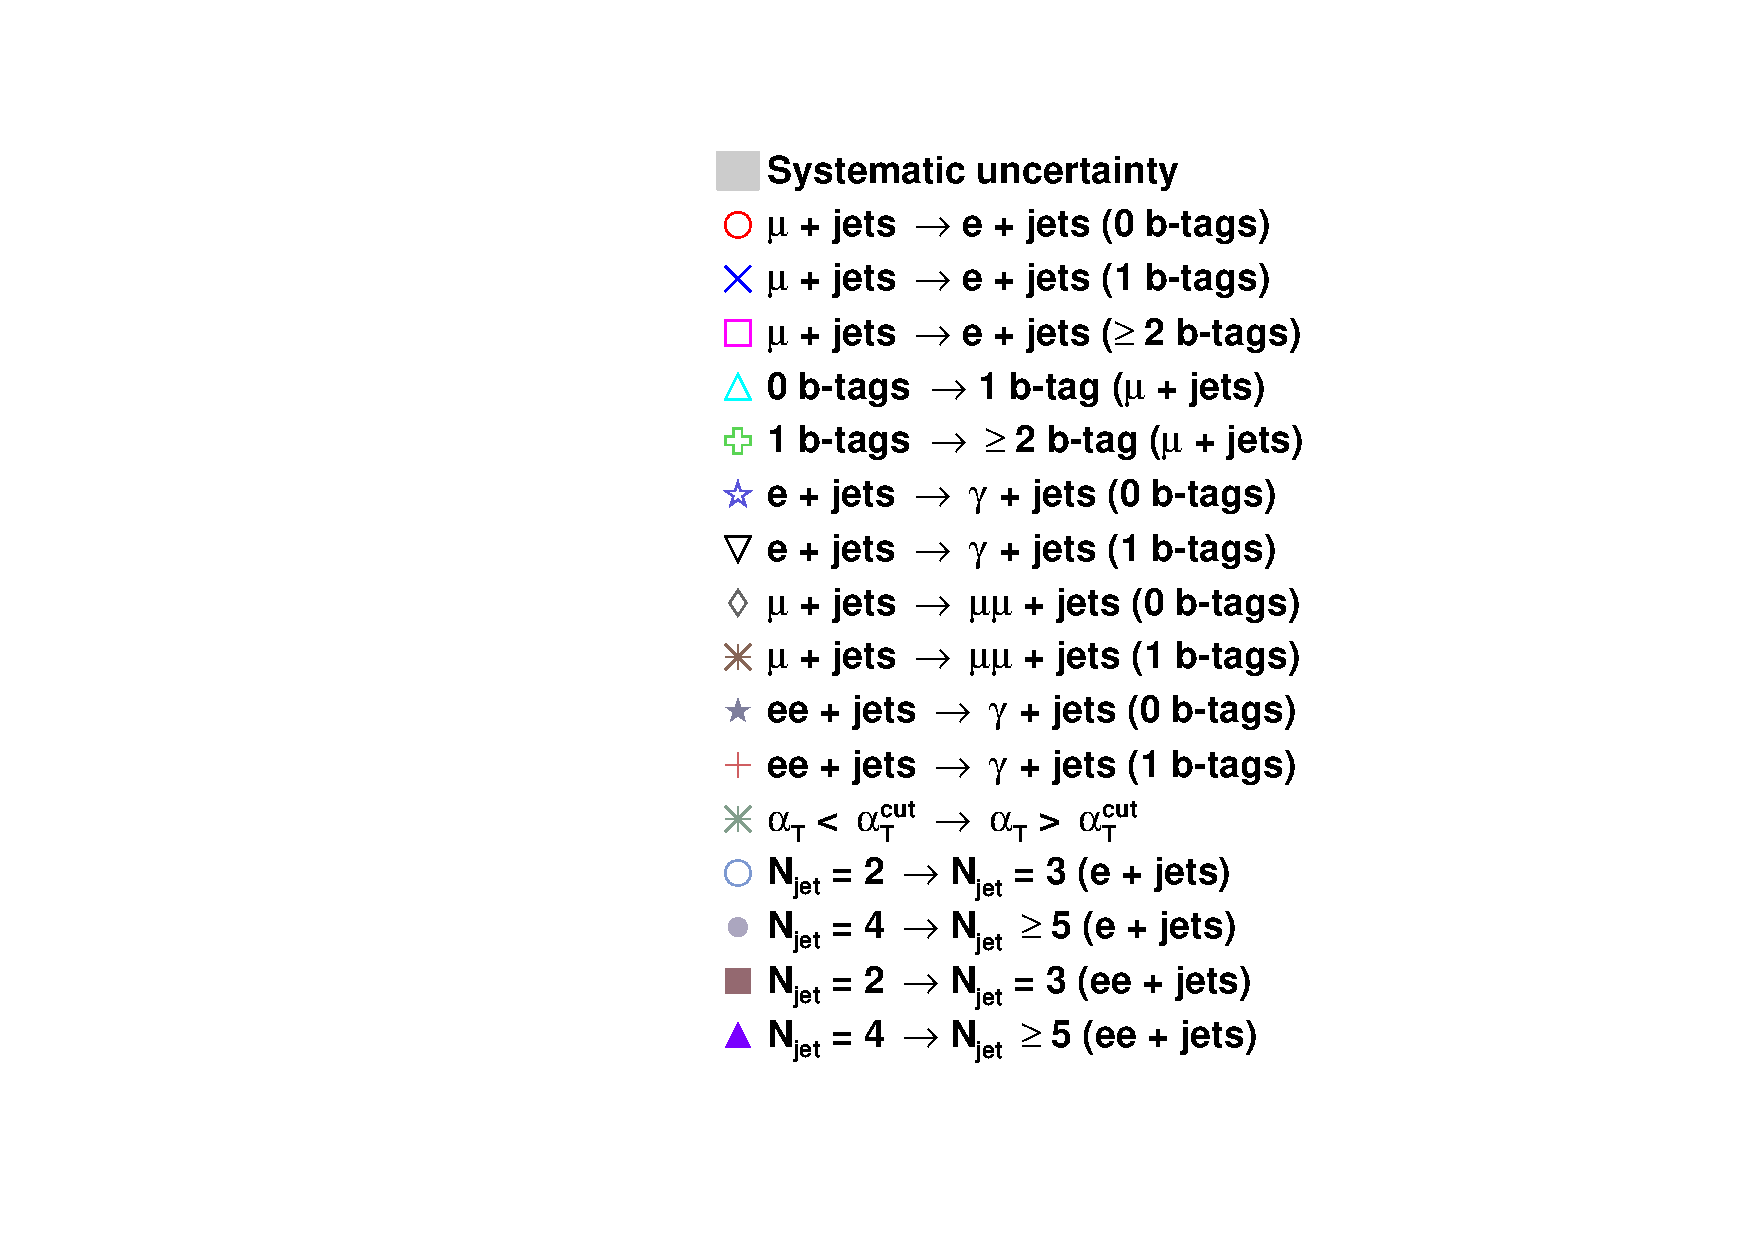
\includegraphics[width=0.4\textwidth]{figures/closureTests/legend.pdf}} \\
    \subfigure[$L_{\rm int} = 3\fbinv, \njet = 4$]{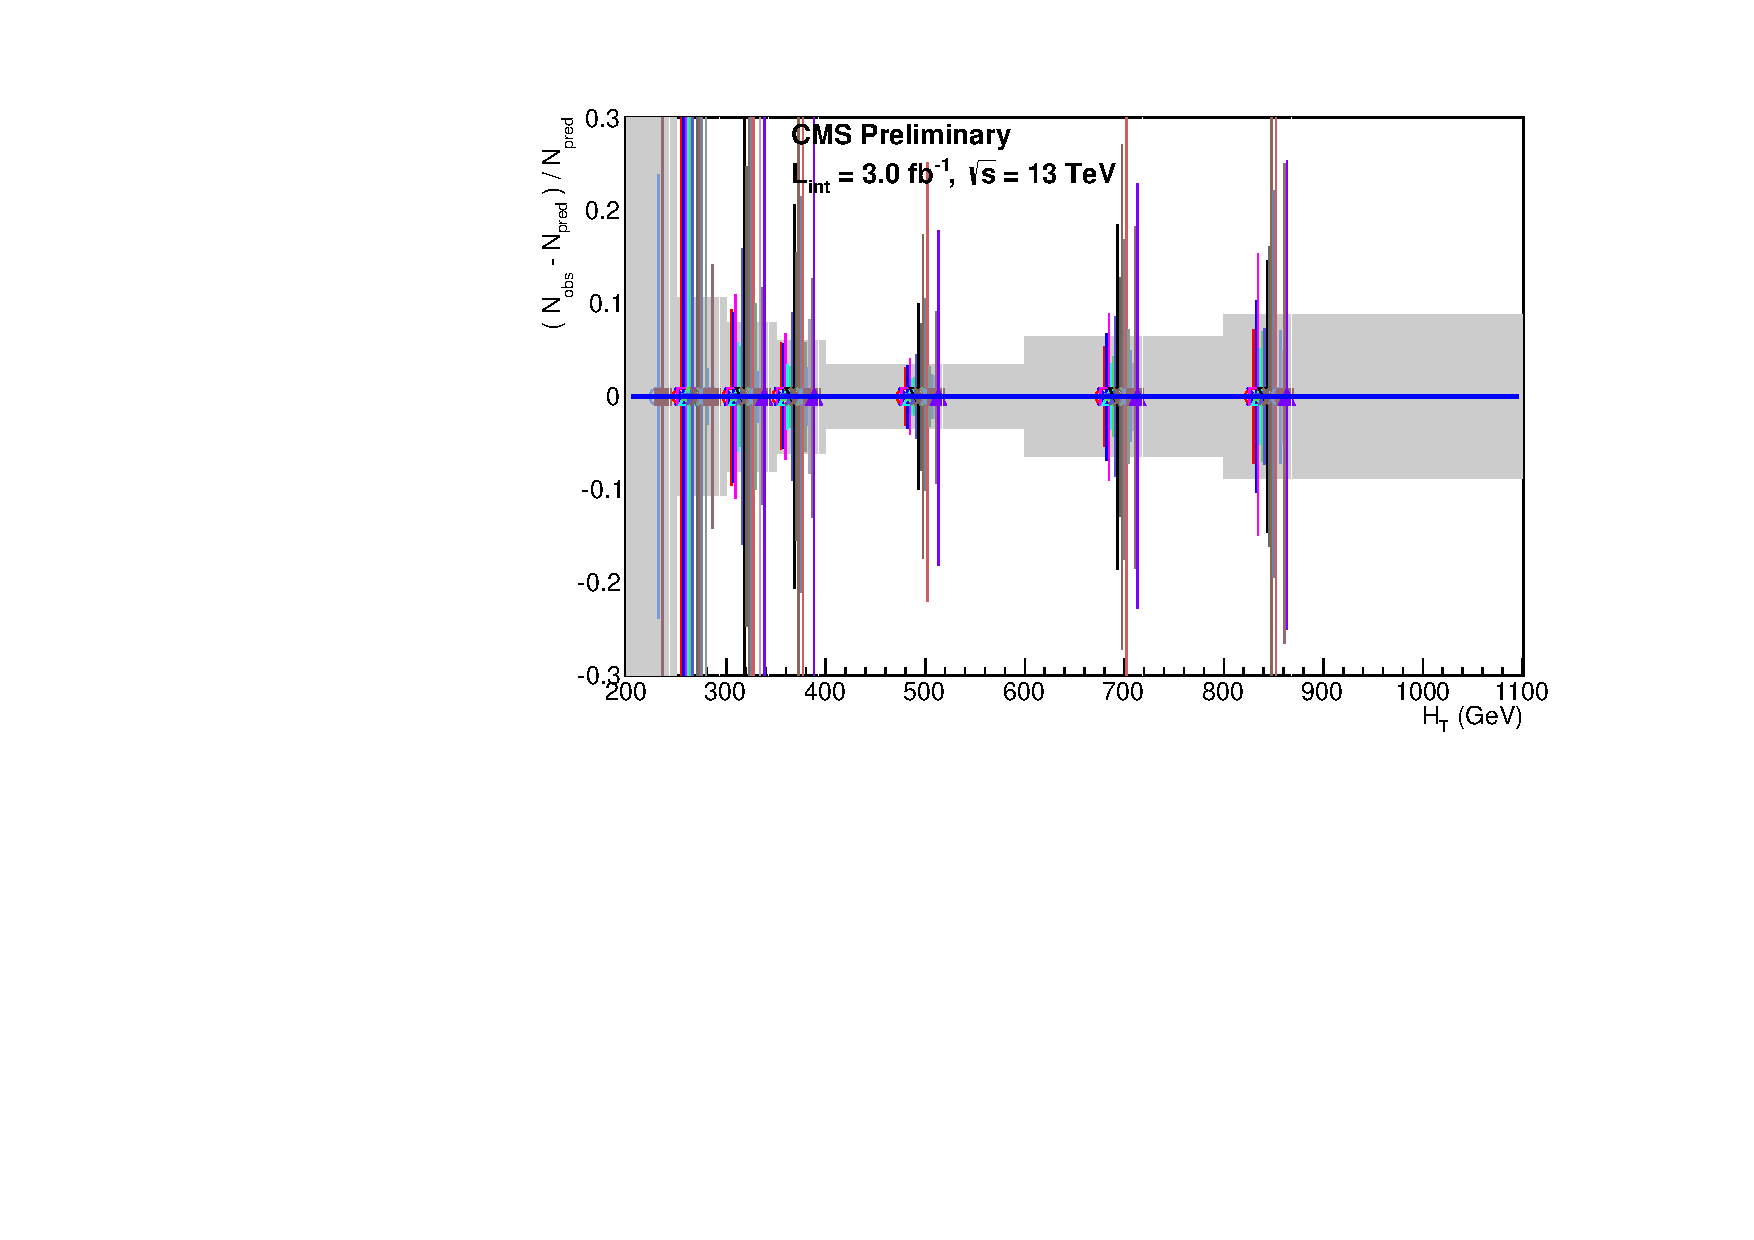
\includegraphics[width=0.5\textwidth]{figures/closureTests/eq4j_lumi3.pdf}} ~~
    \subfigure[$L_{\rm int} = 3\fbinv, \njet \geq 5$]{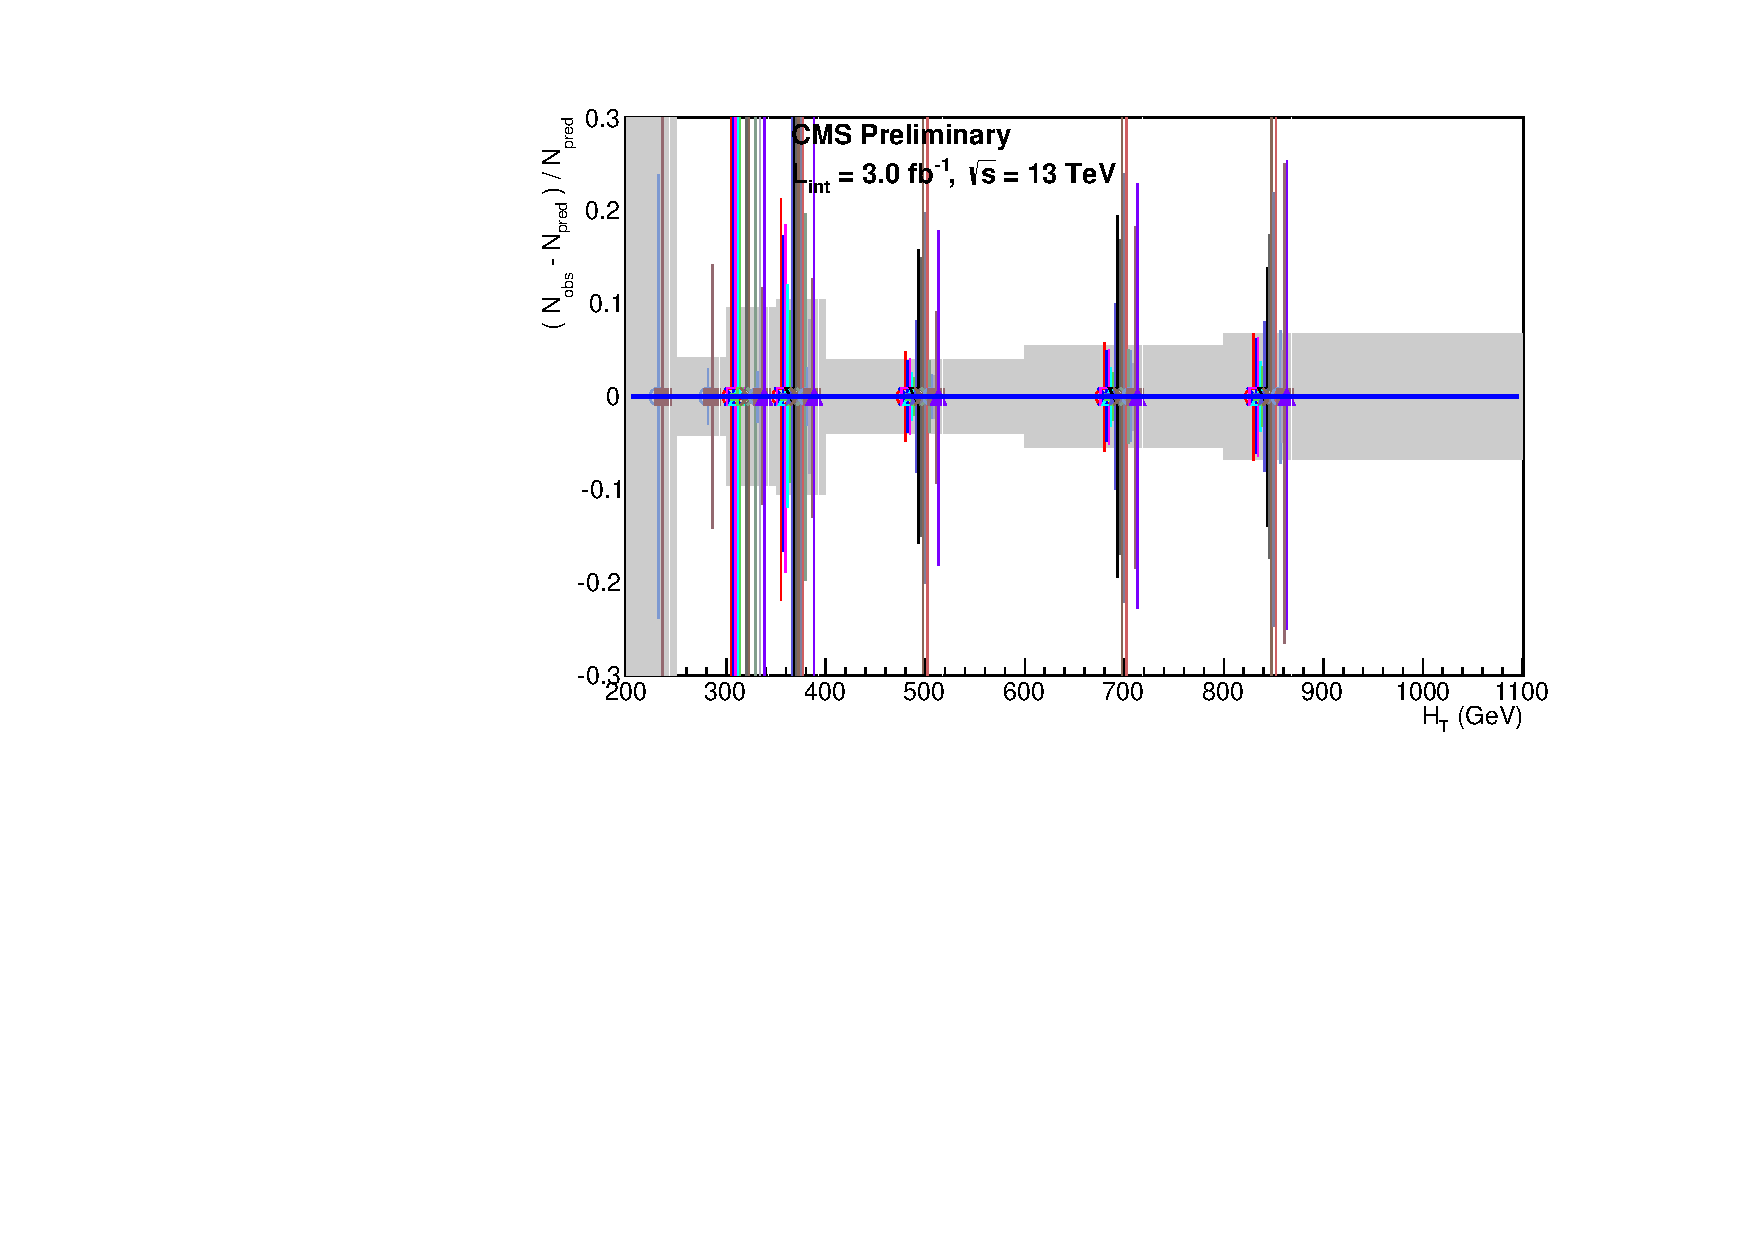
\includegraphics[width=0.5\textwidth]{figures/closureTests/ge5j_lumi3.pdf}} \\
%    \subfigure[$L_{\rm int} = 10\fbinv, \njet = 4$]{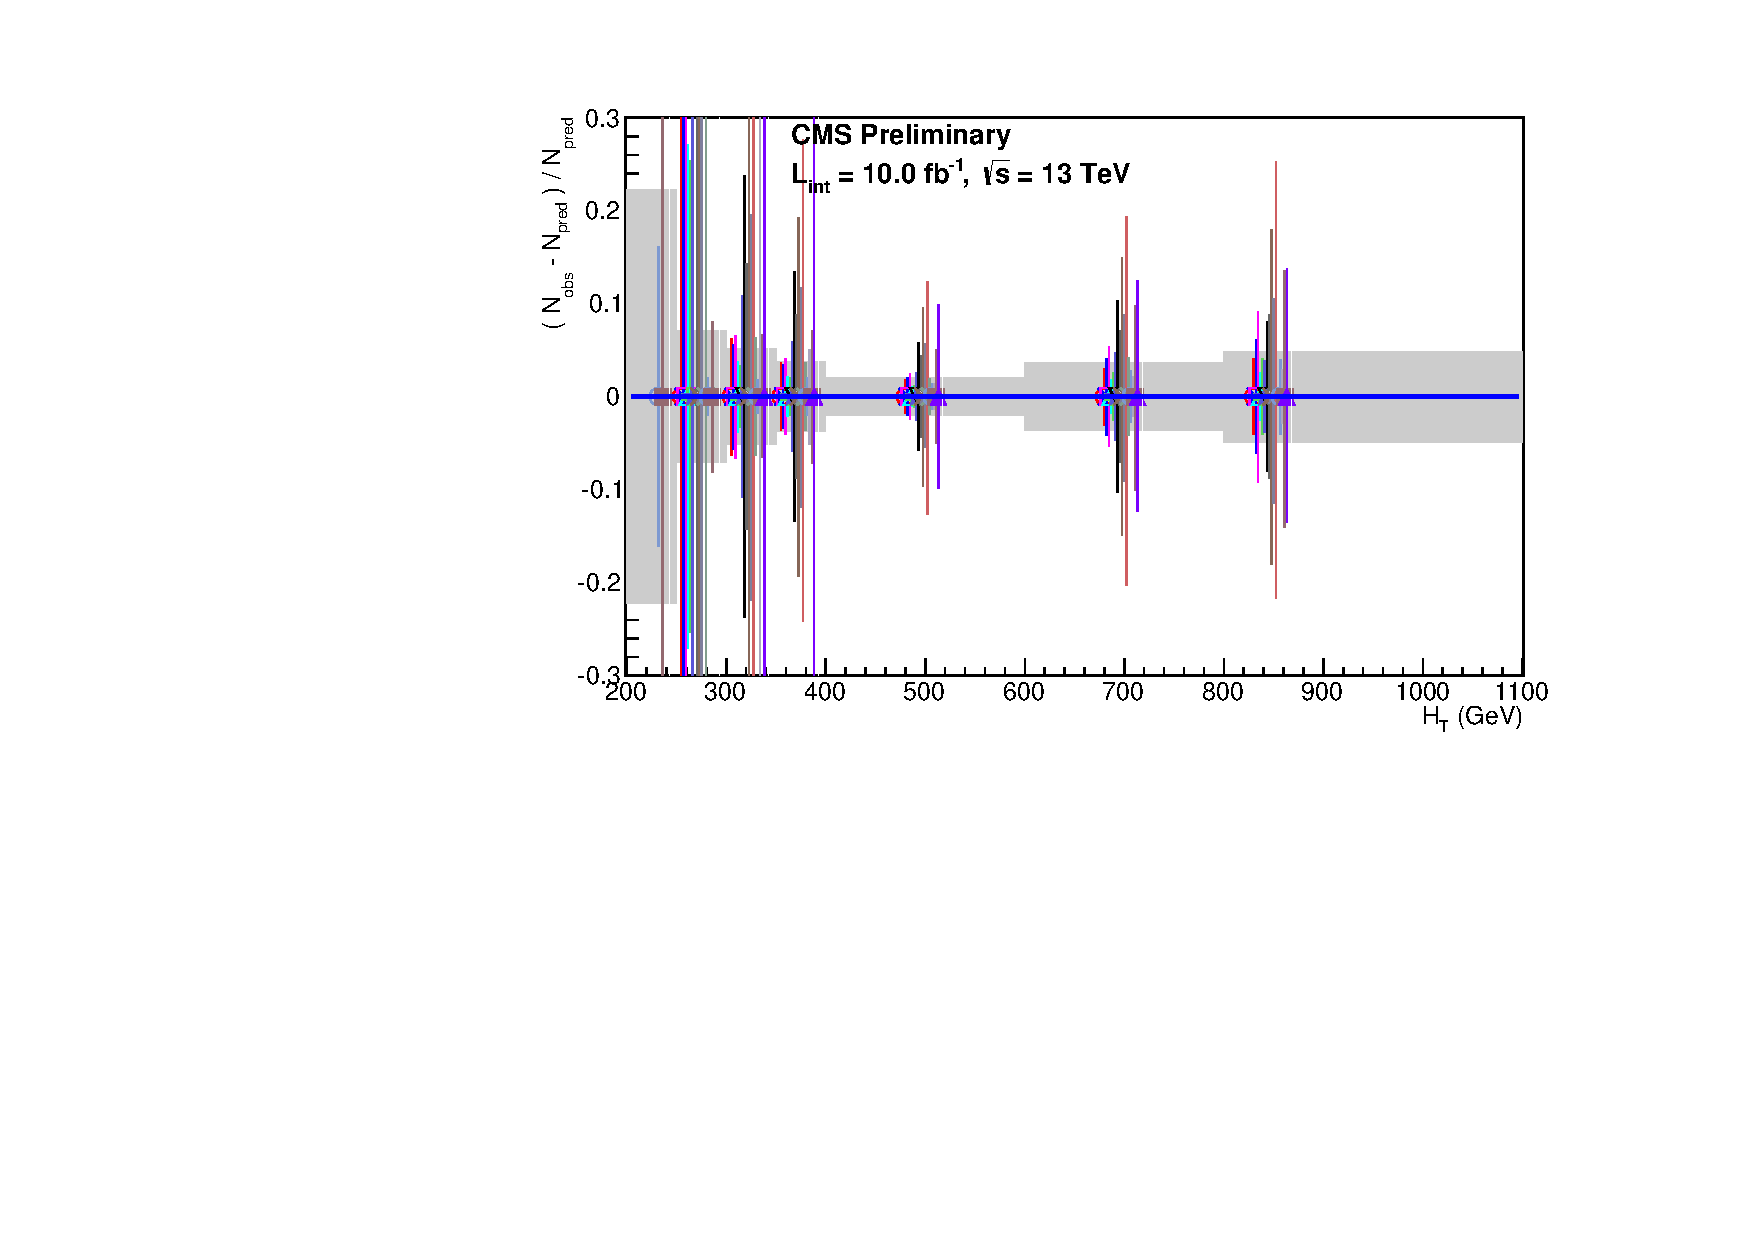
\includegraphics[width=0.5\textwidth]{figures/closureTests/eq4j_lumi10.pdf}} ~~
%    \subfigure[$L_{\rm int} = 10\fbinv, \njet \geq 5$]{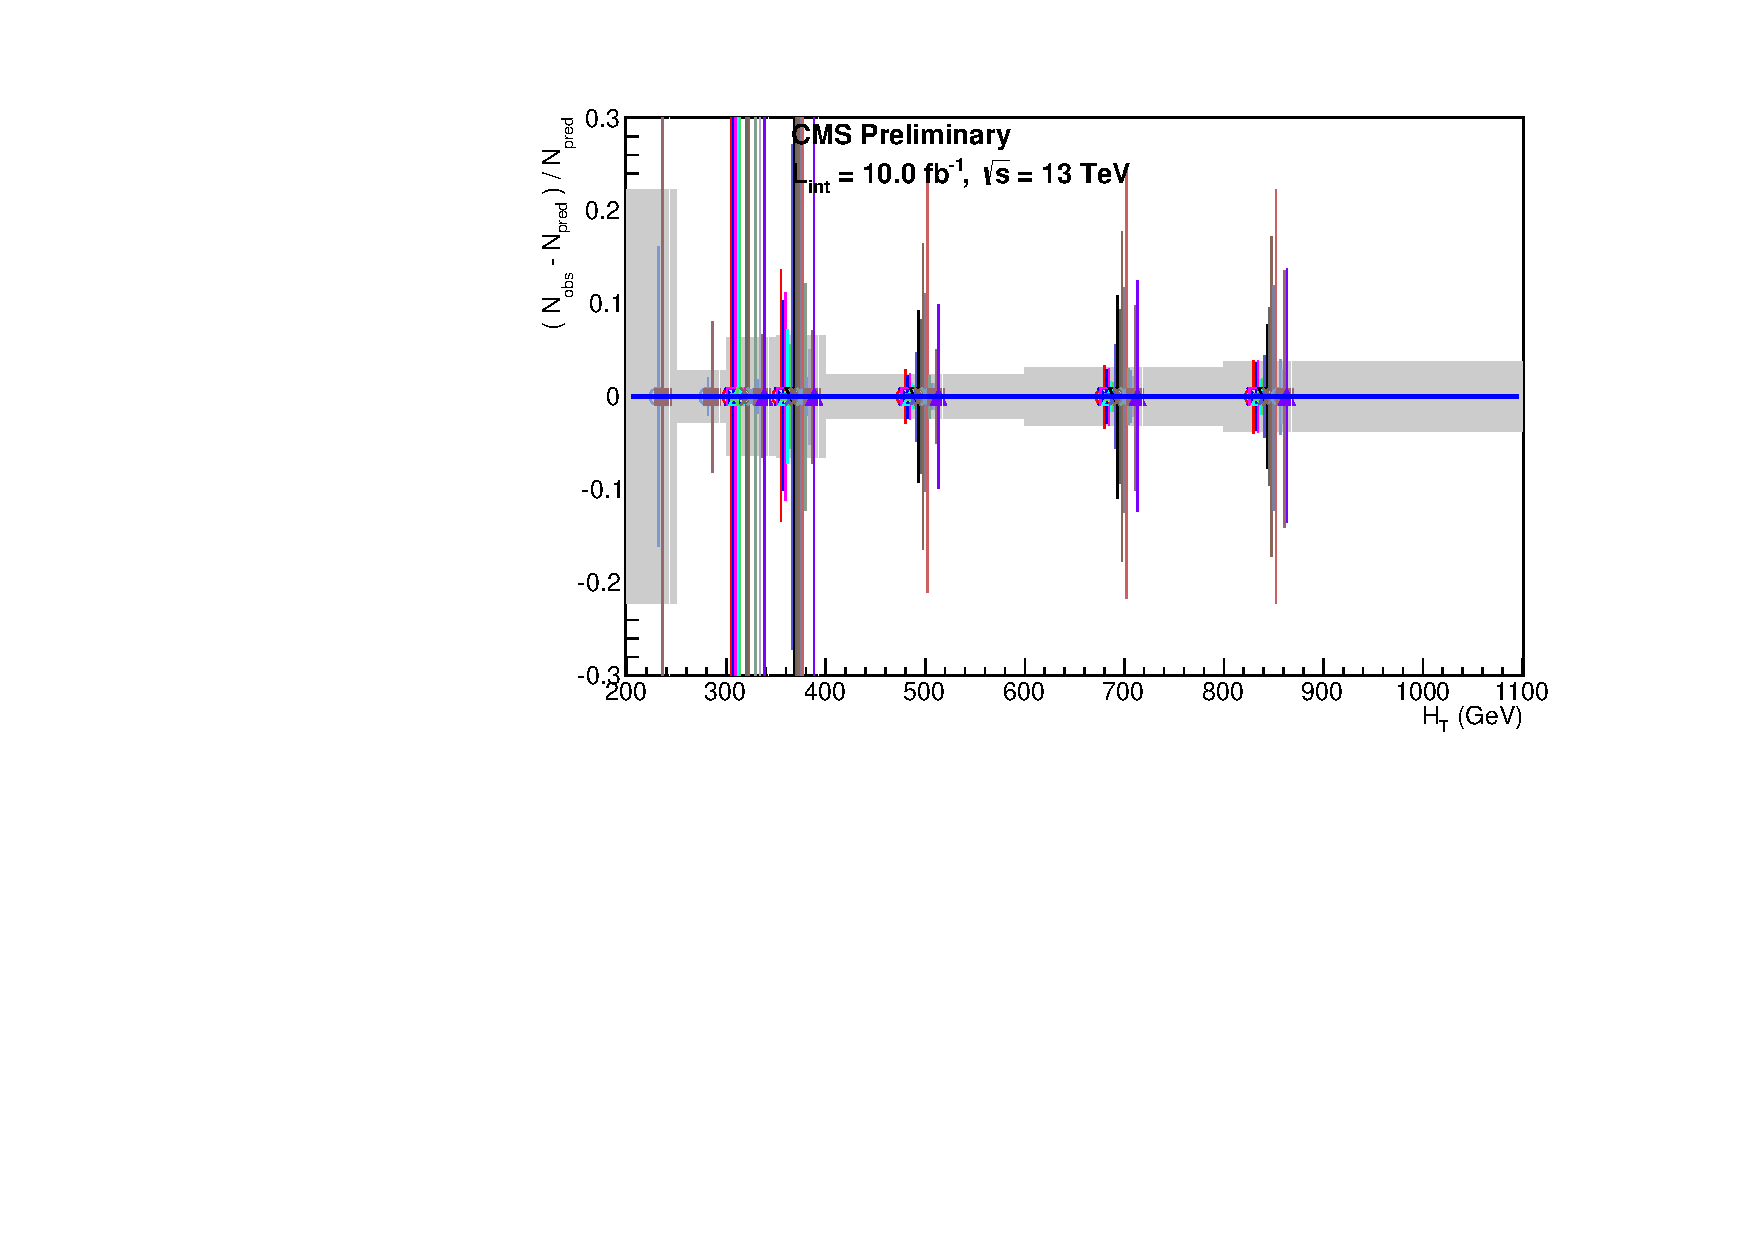
\includegraphics[width=0.5\textwidth]{figures/closureTests/ge5j_lumi10.pdf}} \\
    \caption{Sets of closure tests (open symbols) overlaid on top of
      the systematic uncertainty estimates used for each of the seven
      \scalht bins (shaded bands) for two different jet multiplicity bins (columns).}
    \label{fig:closure}
  \end{center} 
\end{figure}

The first three sets of closure tests are carried out between the \mj
sample and the \ej sample. These cross check the two different lepton
identification efficiencies for three b-tag multiplicity scenarios,
\njet = 0 (red circles), 1 (times symbols) and $\geq$2 (squares).
%% In particular, the 0 b-tag sub-sample is enriched in $W$+jets events, while the $\geq$2 b-tags is very pure in \ttbar.
% The first three sets of closure tests are carried out within the $\mu$
% + jets sample. The first set (indicated by circles) probes the
% modelling of the \alphat distribution in genuine \met events as a
% function of \scalht. This is important to verify the approach of using
% \mj and \mmj samples without an \alphat requirement to make background
% predictions in the signal region, as described in
% Sec.~\ref{sec:larger}. The tests confront data yields in the \mj
% sample with an \alphat requirement against predictions determined in a
% \mj sample with the \alphat requirement inverted. As usual,
% corresponding expectations from simulation are obtained to construct
% the transfer factors required to make the predictions.

The fourth (triangles) and fifth (green crosses) sets probe the
sensitivity of the transfer factors to the relative admixture of
events from the $W$ + jets and \ttbar processes by varying the number
of b-tagged jets within the \mj sample. These tests are conservative,
as the admixture changes little between the \mj sample and the signal
region (as there is no extrapolation in \nb), whereas the closure
tests use sub-samples with different \nb bins and therefore different
admixtures of $W$ + jets and \ttbar events. \eg, the former uses a
$W$-enriched sub-sample (selected by requiring zero b-jets) to predict
yields in a \ttbar-enriched sub-sample (selected by requiring one
b-jet).  These two tests also probe the modelling of the
reconstruction of b-quark jets, although this is addressed more
precisely by dedicated studies involving varying the uncertainties in
b-tag scale factors, as the one performed in the previous analysis,
see for instance \cite{CMS_AN_2013-366}. This study will be repeated
for this analysis.

The sixth (hollow stars) and seventh (inverse triangles) sets deal with
the consistency of the prediction of \wej with $\gamma$ + jets in two
different b-tag multiplicity bins. This is important for understanding
the consistency of the \znunu + jets background predictions from both
\wej and \gj events along with the associated assumptions (such
as the negligible effect of the vector boson mass on kinematic
distributions from the V + jets and \gj samples under sufficient
boost). Additional checks between these two sub-samples (and also
between the single and di-lepton sub-samples) will also be performed
with the charge of the single lepton sample taken into consideration,
which will allow to probe the simulation modelling of acceptance
effects due to $W$ polarisation.

The eighth (diamonds) and ninth (brown asterisks), connecting the $\mu$
+ jets and $\mu\mu$ + jets control samples for two different \nb~bins
(zero and one) address the modelling of vector boson production
(including the handling of contamination from \ttbar). The muon
trigger and reconstruction efficiencies are also probed, given that
exactly one and two muons are required in the two control
samples. However, dedicated data-driven methods are used to measure
the muon trigger and reconstruction efficiencies, with values taken
from the muon POG.

The tenth (solid stars) and eleventh (red crosses) deal with the
consistency between the \zee + jets and $\gamma$ + jets
samples, which is a further check on the validity of using the \gj
process to predict the \znunu\, + jets process.

The twelfth set of tests (indicated by green asterisks) probes the
modelling of the \alphat distribution in genuine \met events as a
function of \scalht. This is important to verify the approach of using
\mj, \ej, \mmj, and \eej samples without an \alphat requirement to
make background predictions in the signal region. The tests confront
data yields in the \mj sample with an \alphat requirement against
predictions determined in a \mj sample with the \alphat requirement
inverted. As usual, corresponding expectations from simulation are
obtained to construct the transfer factors required to make the
predictions.

The final four sets of tests probe the simulation modelling of jet
multiplicity in the \ej (blue open circles and grey closed circles),
and \eej (brown closed squares and blue closed triangles) samples,
which is checked due to the exclusive binning in jet multiplicity.  As
in the case of the $W$ + jets / \ttbar admixture, these sets of tests
are a conservative check, as predictions are always made from the same
jet multiplicity bin, whereas the closure tests translate between the
two bins.

The aforementioned closure tests are not the only ones considered or
checked, \ie, the list above is not exhaustive. However, they are a
representative set that cover the main potential sources of bias in
the transfer factors derived from simulation. 

\subsection{Systematic uncertainties in the transfer
factors\label{sec:syst-from-closurei-3fb}}

For the MC studies detailed in Sec.~\ref{sec:closure-mc-study}, this 
procedure yields the values quoted in
Fig.~\ref{fig:systematics}, which shows the systematic uncertainty
on the transfer factor as a function of the \scalht and (\nb,\njet)
category, extracted for 3 \ifb of integrated luminosity. These are
calculated with the procedure defined in
Sec.~\ref{sec:syst-from-closure}.
%and 10 \ifb. 

\begin{figure}[]
  \centering
  \subfigure[Systematic uncertainties for 3 \ifb]{
    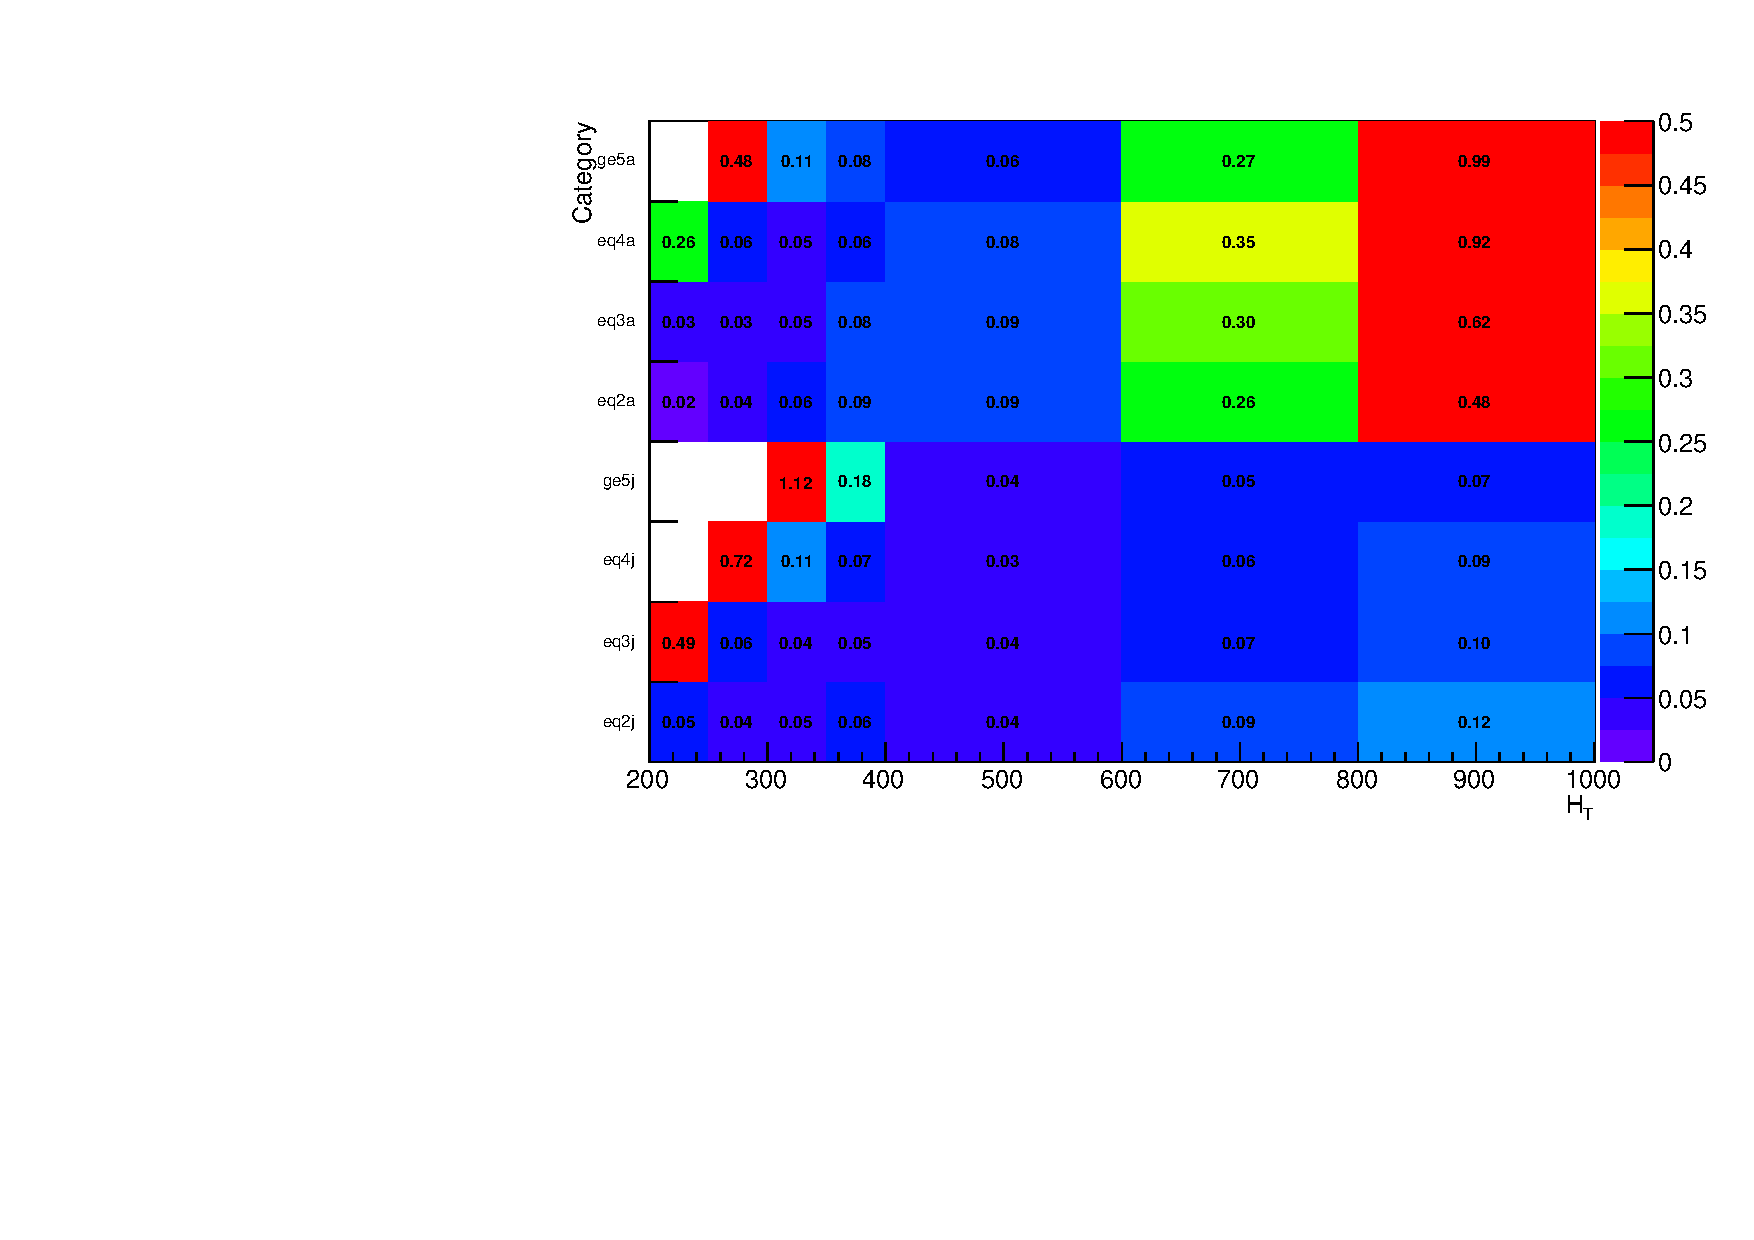
\includegraphics[width=0.8\textwidth]{figures/closureTests/systOut2d3fb.pdf}
  }
%  \subfigure[Systematic uncertainties for 10 \ifb]{
%    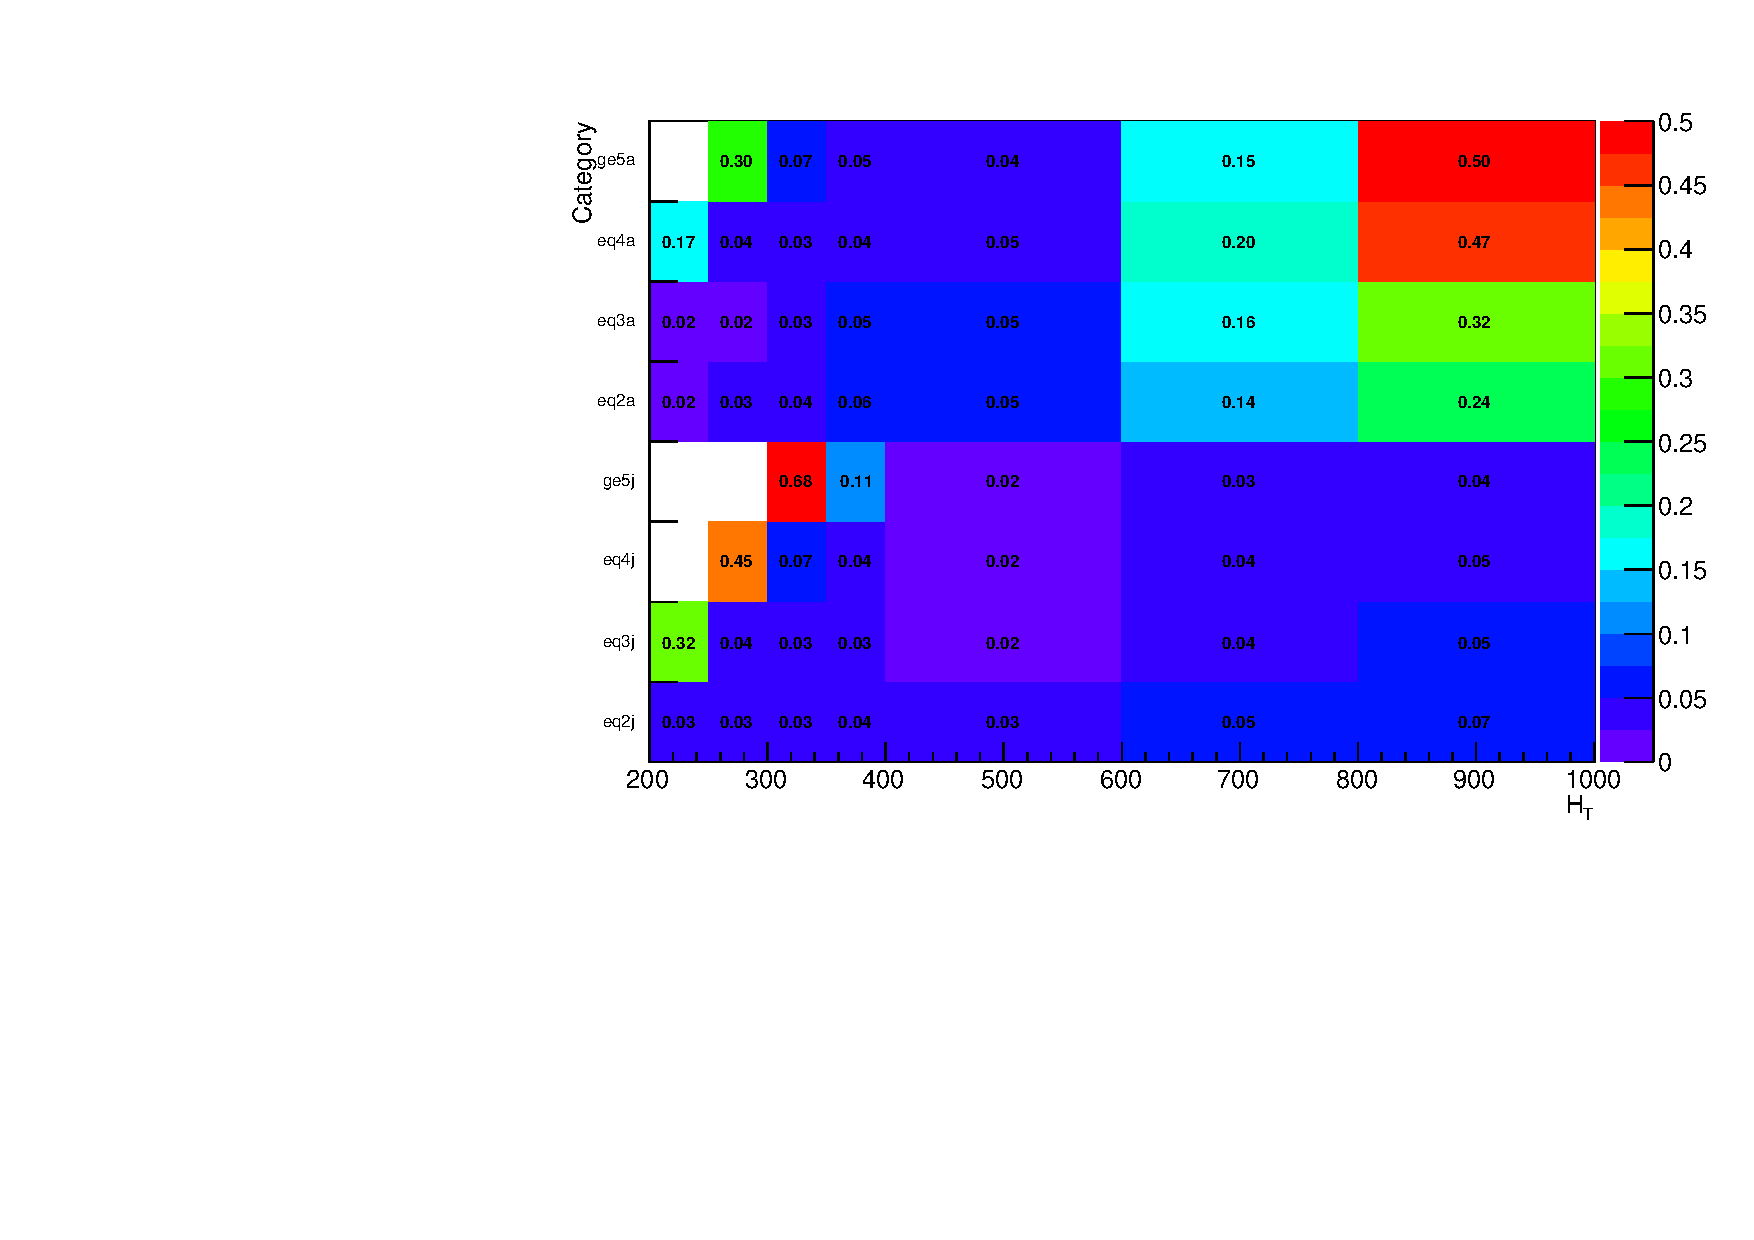
\includegraphics[width=0.5\textwidth]{figures/closureTests/systOut2d10fb.pdf}
%  }
  \caption{\label{fig:systematics} Expected systematics derived from the closure tests shown for
the 3 \ifb.}
\end{figure}

\subsection{Splitting up the closure tests based on background
processes \label{sec:closure-split}}

In Fig.~\ref{fig:ttWClosure} the closure tests selected for the $W$ and
\ttbar backgrounds are presented. The exact tests are detailed
in the legend. As the single lepton control samples are used for $W$ and
\ttbar background prediction, closure tests using only these samples
are selected. In addition to the tests described in
Sec~\ref{sec:closure-tests-desc}, closure tests probing the b-tag
extrapolation (hollow star and inverted triangle) are carried out with 
the single electron control sample, analagous to those in the muon control sample.

In Fig.~\ref{fig:ZinvClosure} the closure tests selected for the
\znunu background are presented. For the \znunu prediction, single
lepton, double lepton and the photon control samples are all used.
Closure tests are therefore chosen that test the extrapolation
between these different samples with different b-tag multiplicities. 
These are the first ten closure tests in the legend. Most of these
tests are taken from those in Sec.~\ref{sec:closure-tests-desc}. On top
of these are \mmj to \gj tests (brown asterisk and grey star), analagous to
the \eej to \gj closure tests, and \ej to \eej tests (inverted
triangle and hollow diamond), analagous to the \mj to \mmj tests.

To further probe the use of the single lepton control samples for the
\znunu background prediction, $\mu^+$ to $\mu^-$ and $e^+$ to $e^-$
closure tests are added (red plus and green asterisk). These are 
designed to identify any source of systematic caused by $W$ polarisation 
effects, as discussed in App.~\ref{app:zInvBgControl}.

\begin{figure}[h!]
  \begin{center}
    \subfigure[Legend]{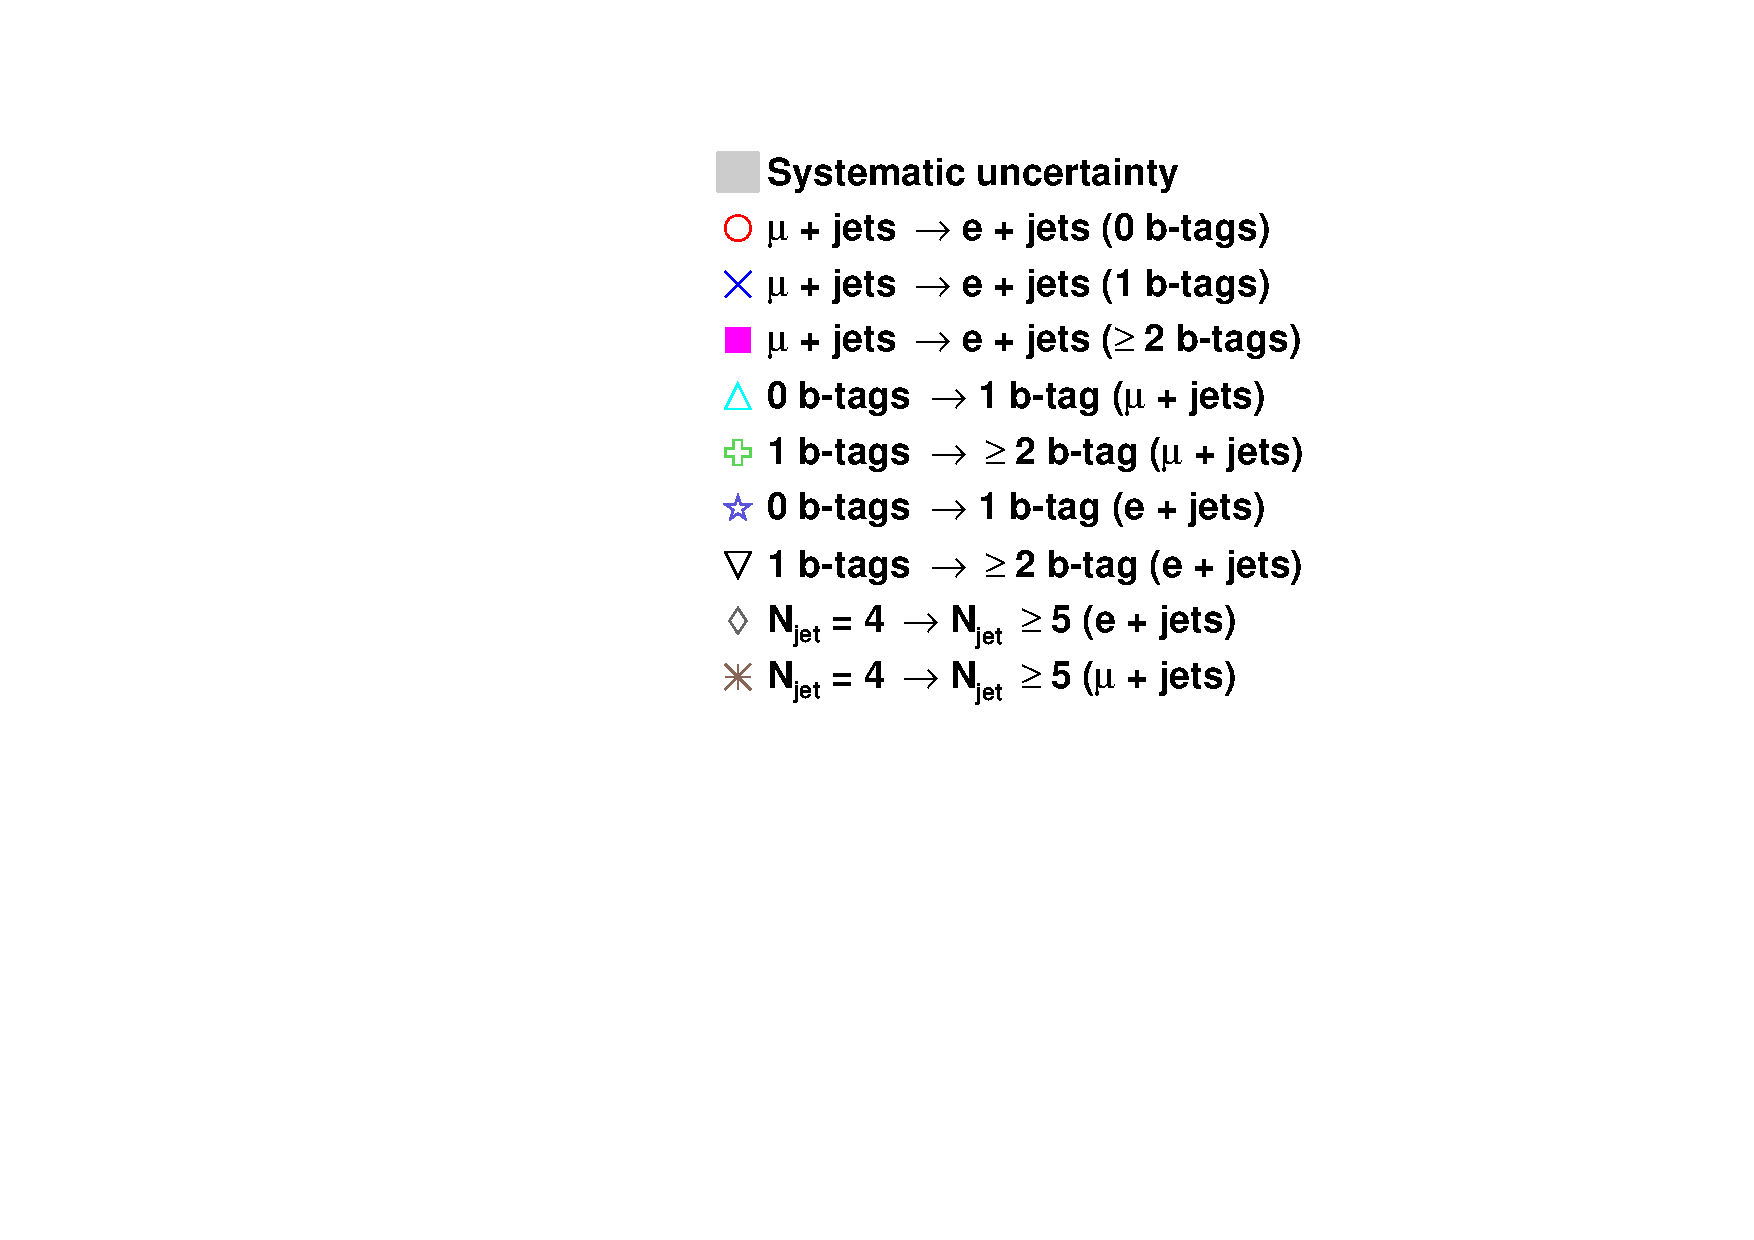
\includegraphics[width=0.4\textwidth]{figures/closureTests/split/ttW/legend.pdf}} \\
    \subfigure[$L_{\rm int} = 3\fbinv, \njet = 4$]{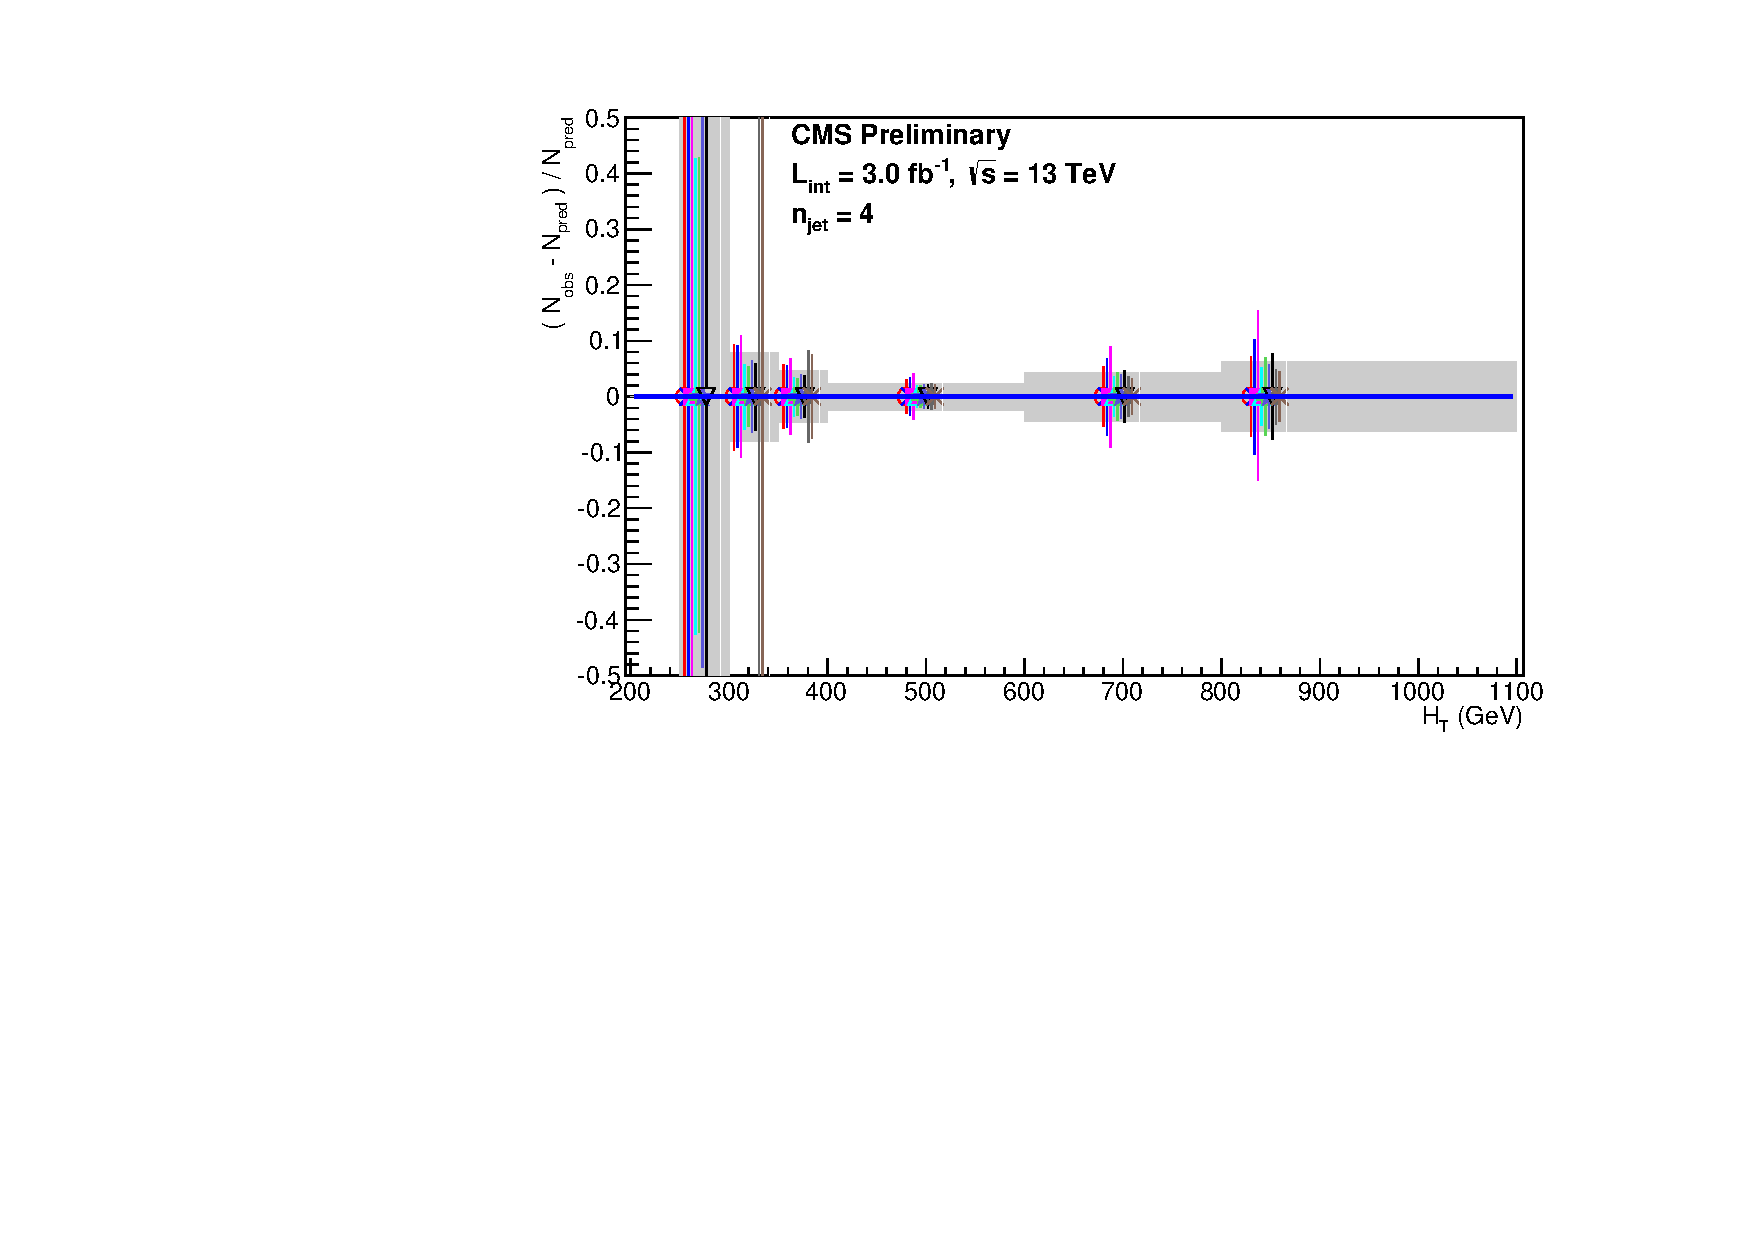
\includegraphics[width=0.5\textwidth]{figures/closureTests/split/ttW/eq4j_lumi3.pdf}} ~~
    \subfigure[$L_{\rm int} = 3\fbinv, \njet \geq 5$]{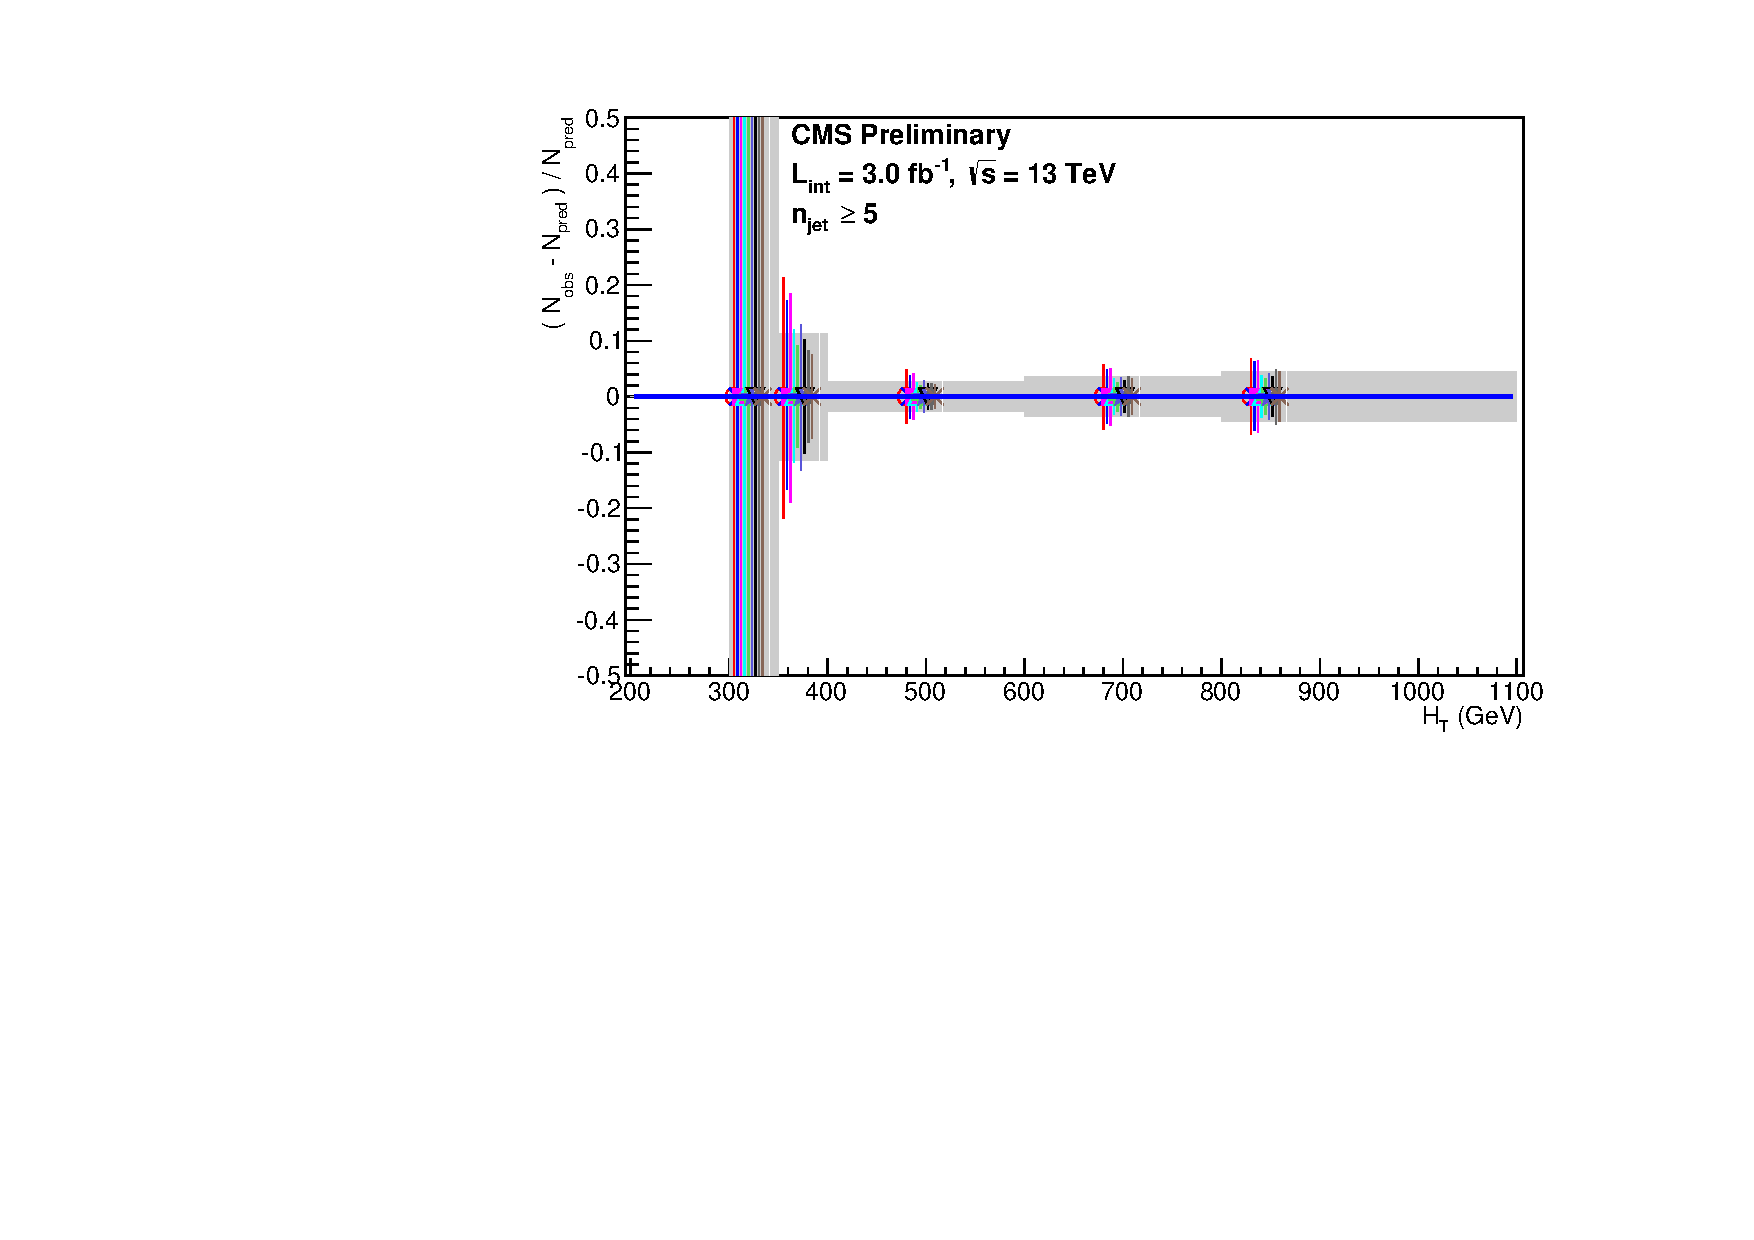
\includegraphics[width=0.5\textwidth]{figures/closureTests/split/ttW/ge5j_lumi3.pdf}} \\
%    \subfigure[$L_{\rm int} = 10\fbinv, \njet = 4$]{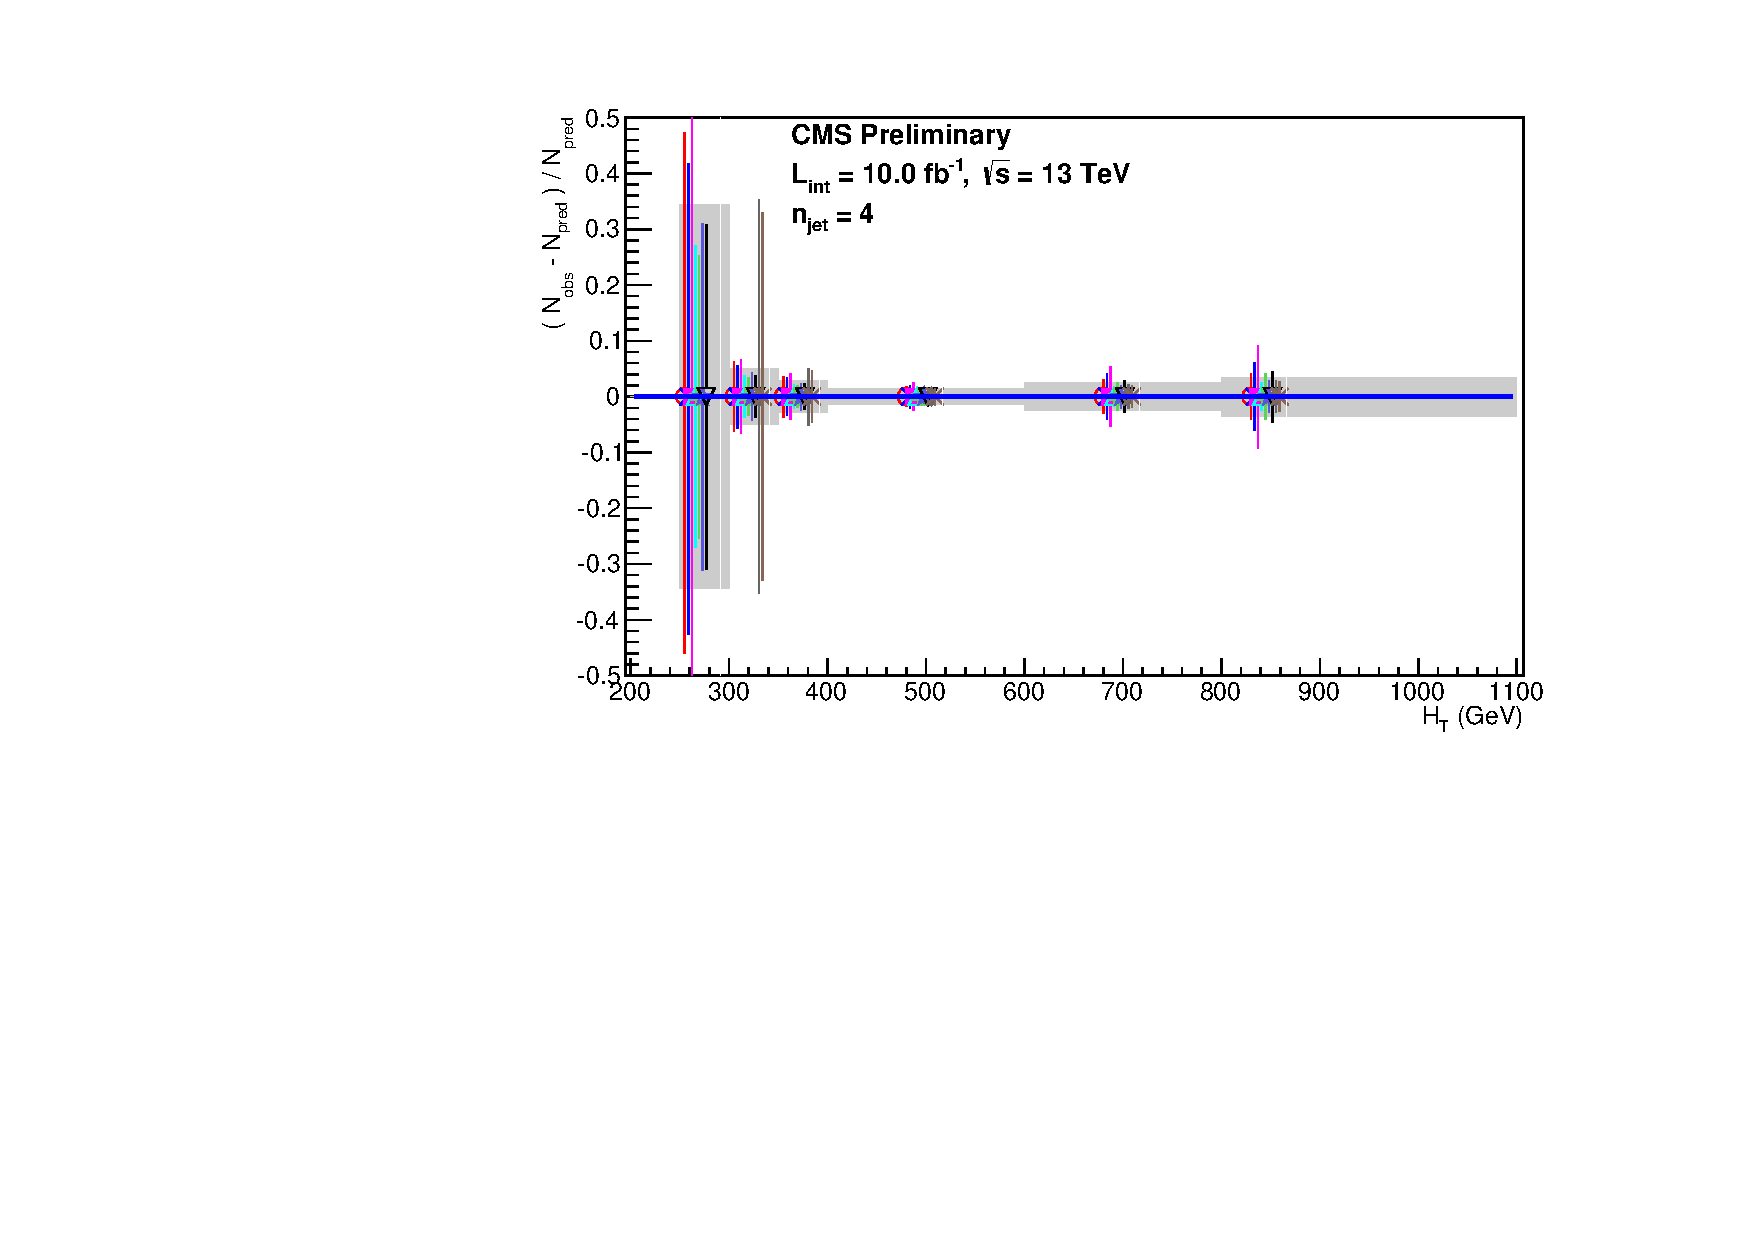
\includegraphics[width=0.5\textwidth]{figures/closureTests/split/ttW/eq4j_lumi10.pdf}} ~~
%    \subfigure[$L_{\rm int} = 10\fbinv, \njet \geq 5$]{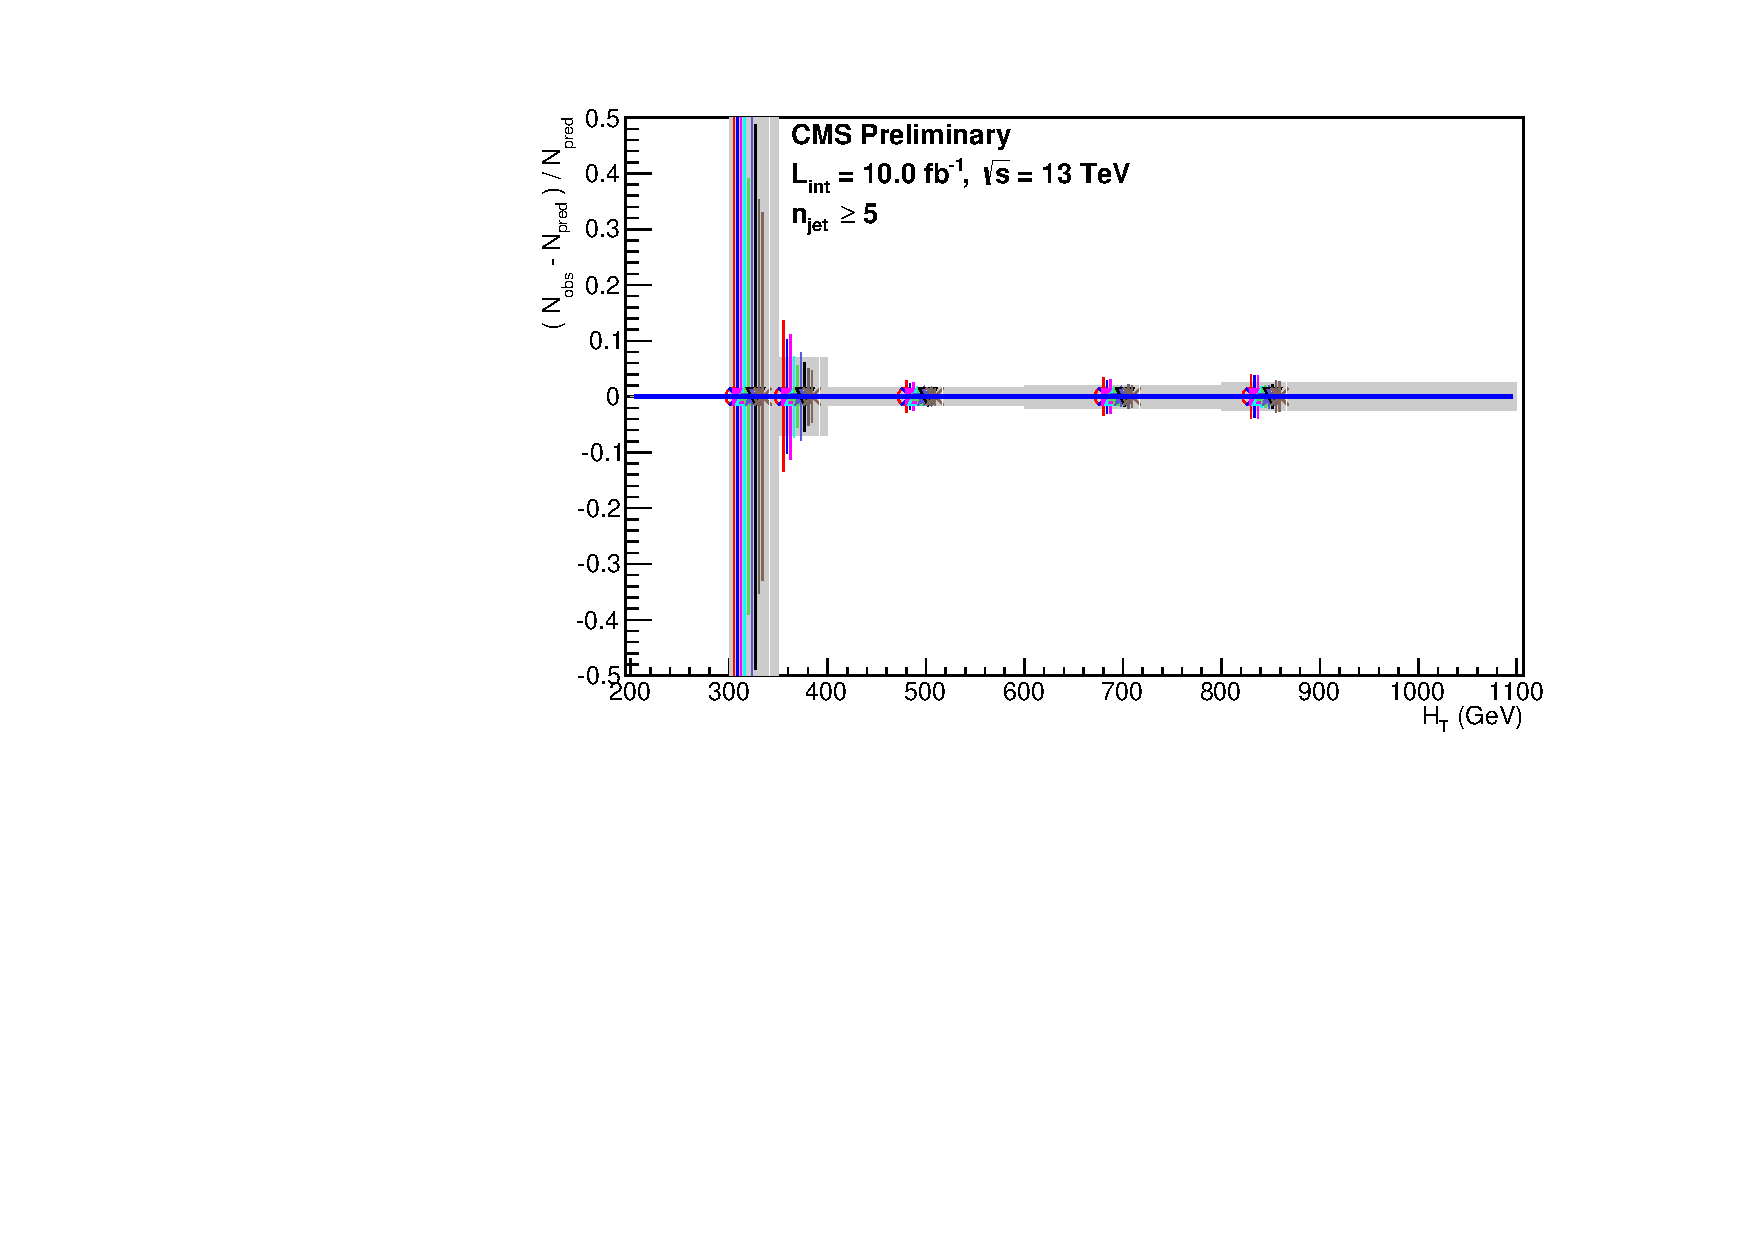
\includegraphics[width=0.5\textwidth]{figures/closureTests/split/ttW/ge5j_lumi10.pdf}} \\
    \caption{Sets of closure tests chosen to probe the $W$ and \ttbar
      background prediction. Each test is overlaid on top of
      the systematic uncertainty estimates used for each of the seven
      \scalht bins (shaded bands), for two different jet
      multiplicity bins (columns).}
    \label{fig:ttWClosure}
  \end{center} 
\end{figure}

\begin{figure}[h!]
  \begin{center}
    \subfigure[Legend]{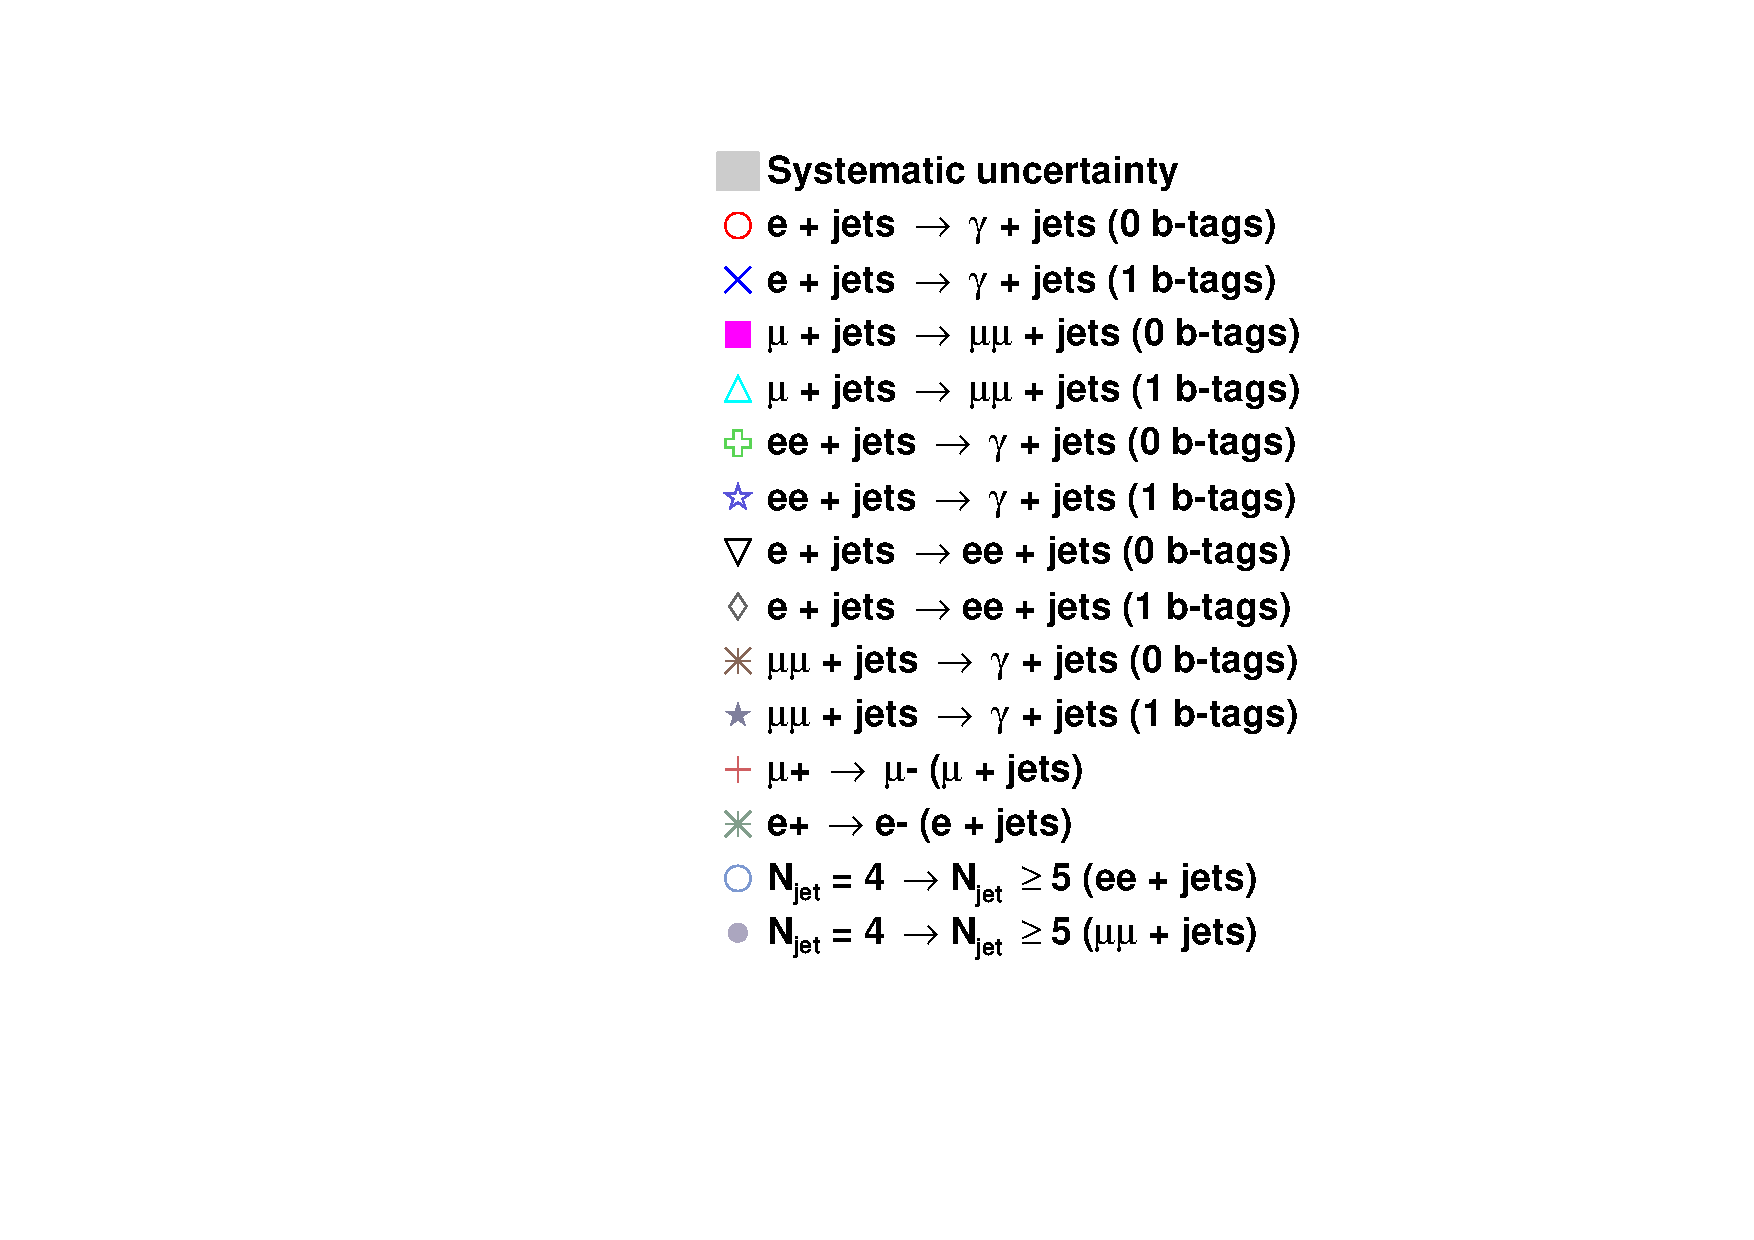
\includegraphics[width=0.4\textwidth]{figures/closureTests/split/Zinv/legend.pdf}} \\
    \subfigure[$L_{\rm int} = 3\fbinv, \njet = 4$]{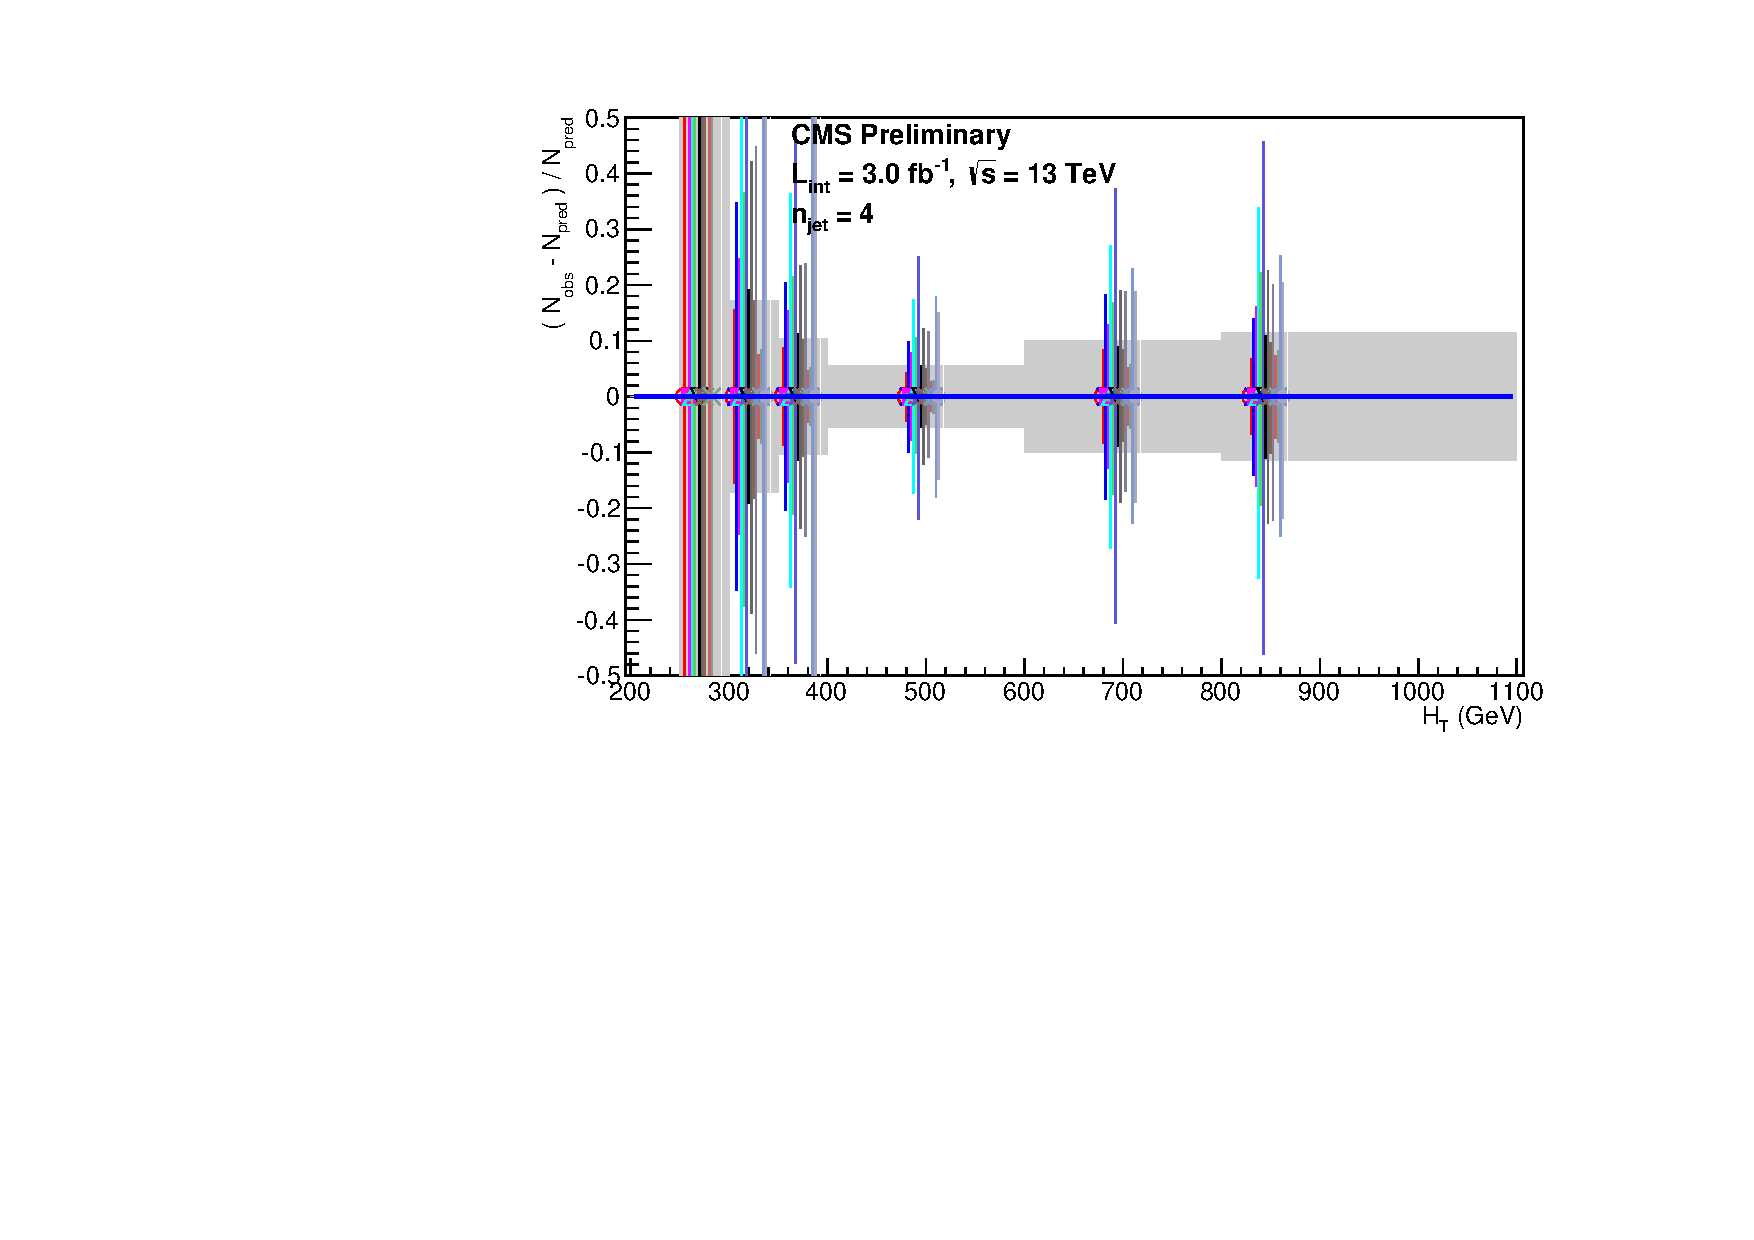
\includegraphics[width=0.5\textwidth]{figures/closureTests/split/Zinv/eq4j_lumi3.pdf}} ~~
    \subfigure[$L_{\rm int} = 3\fbinv, \njet \geq 5$]{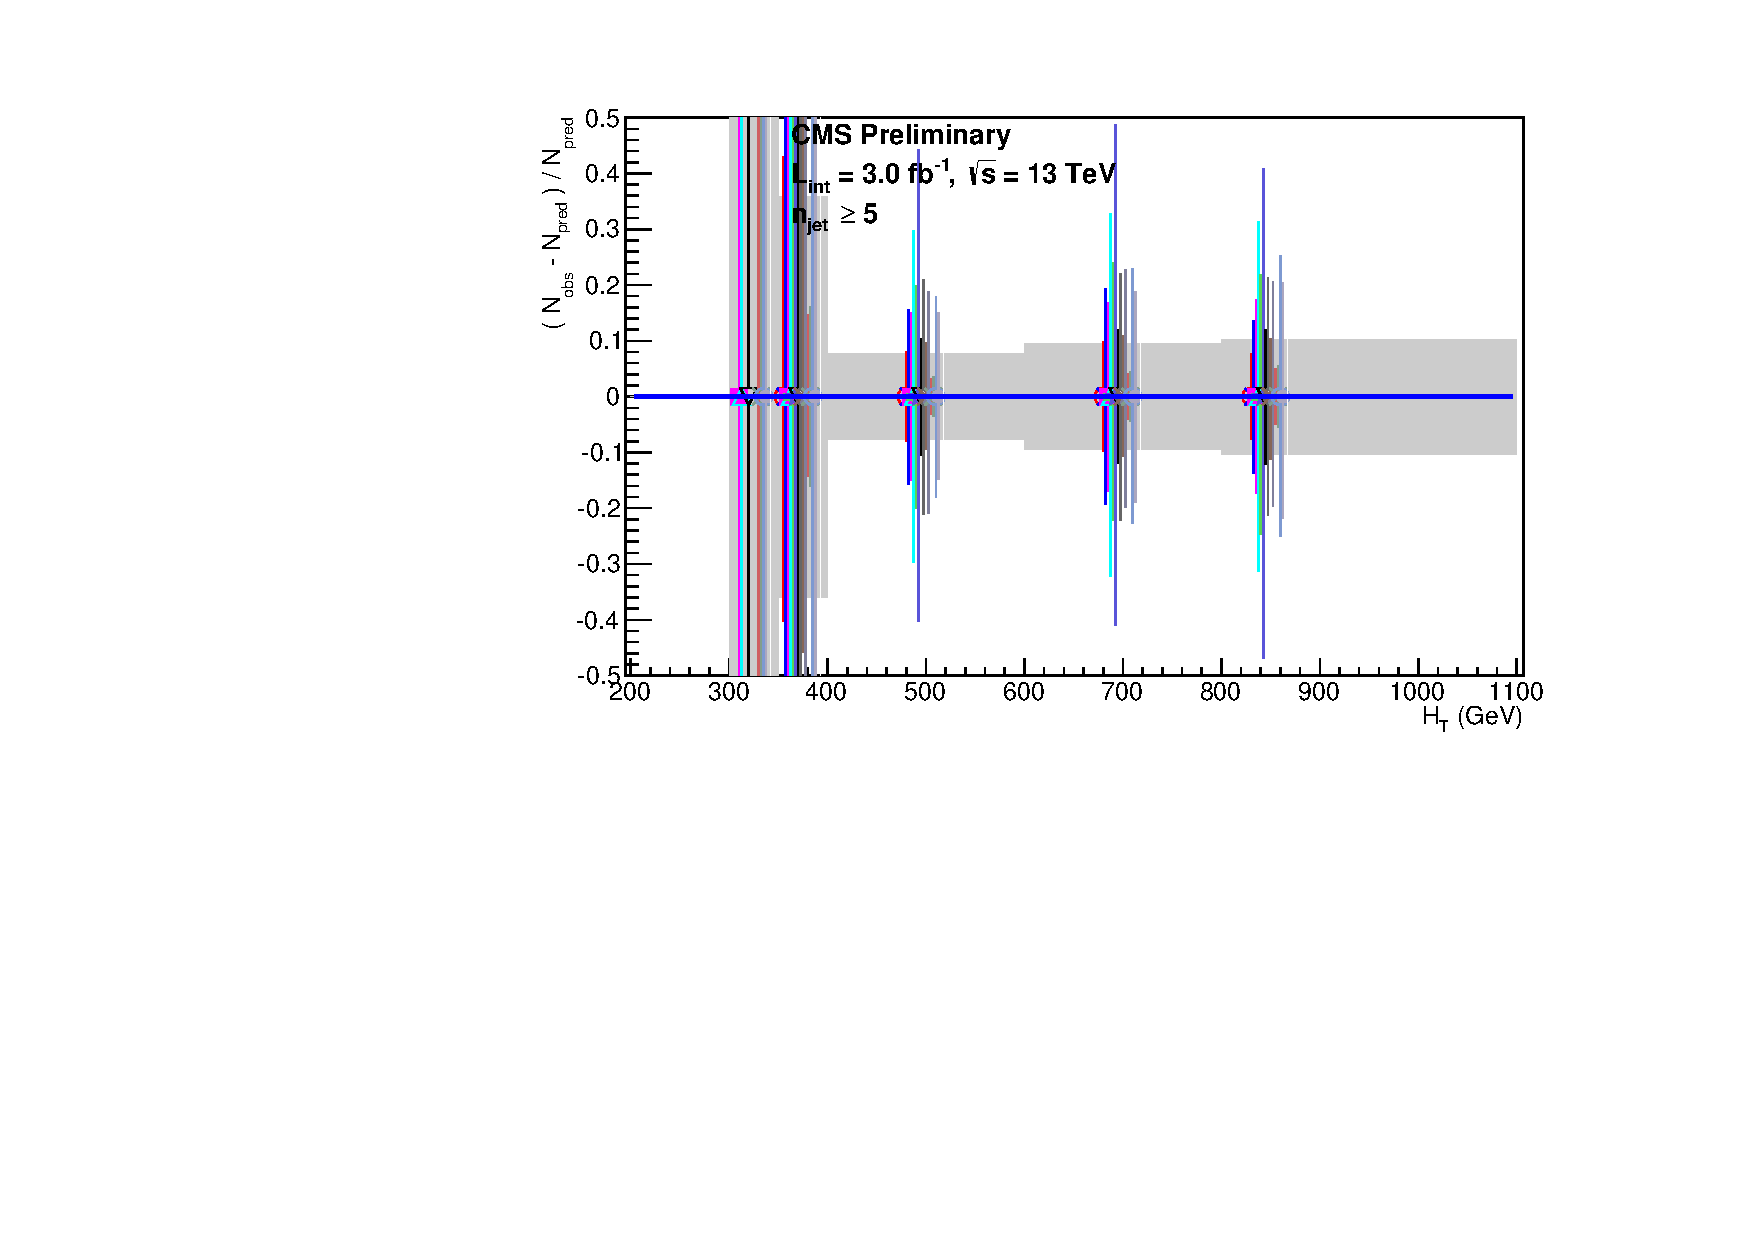
\includegraphics[width=0.5\textwidth]{figures/closureTests/split/Zinv/ge5j_lumi3.pdf}} \\
%    \subfigure[$L_{\rm int} = 10\fbinv, \njet = 4$]{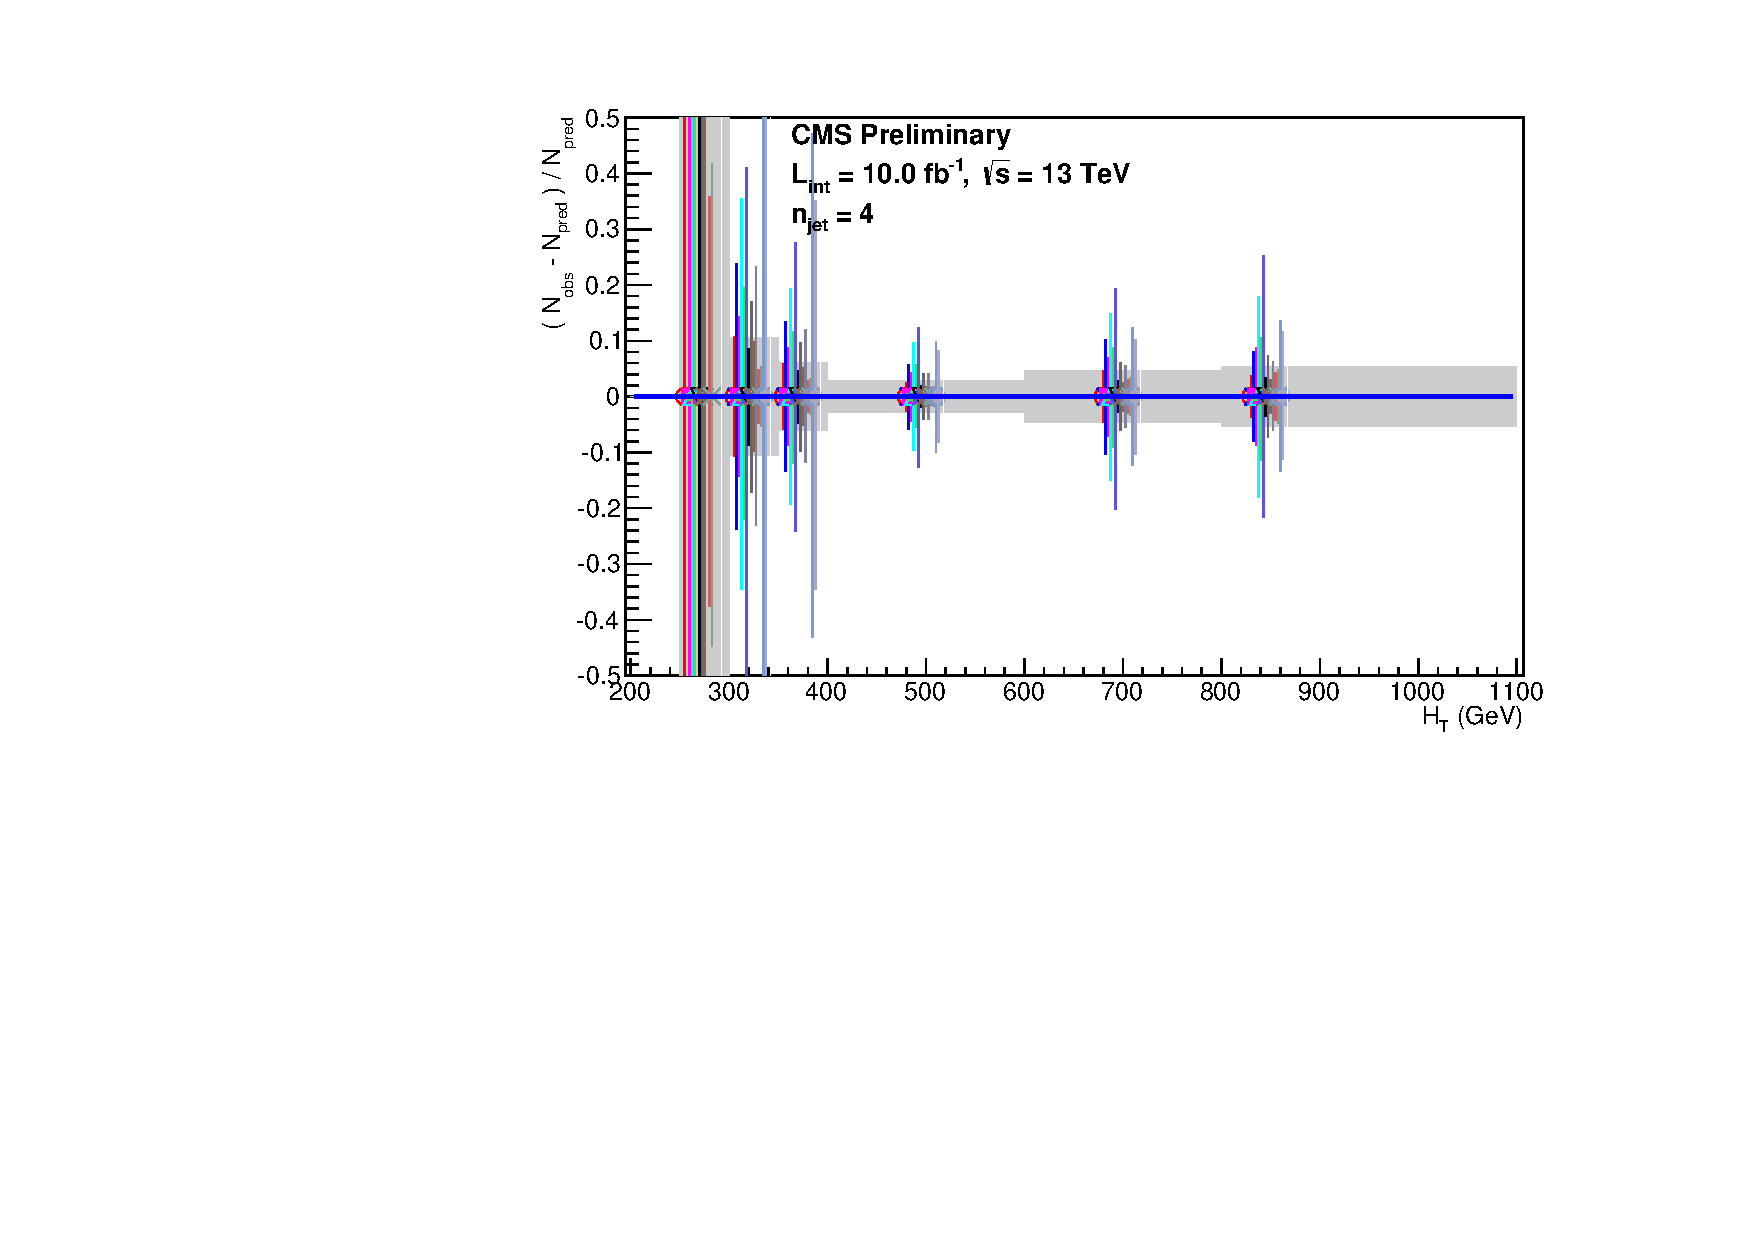
\includegraphics[width=0.5\textwidth]{figures/closureTests/split/Zinv/eq4j_lumi10.pdf}} ~~
%    \subfigure[$L_{\rm int} = 10\fbinv, \njet \geq 5$]{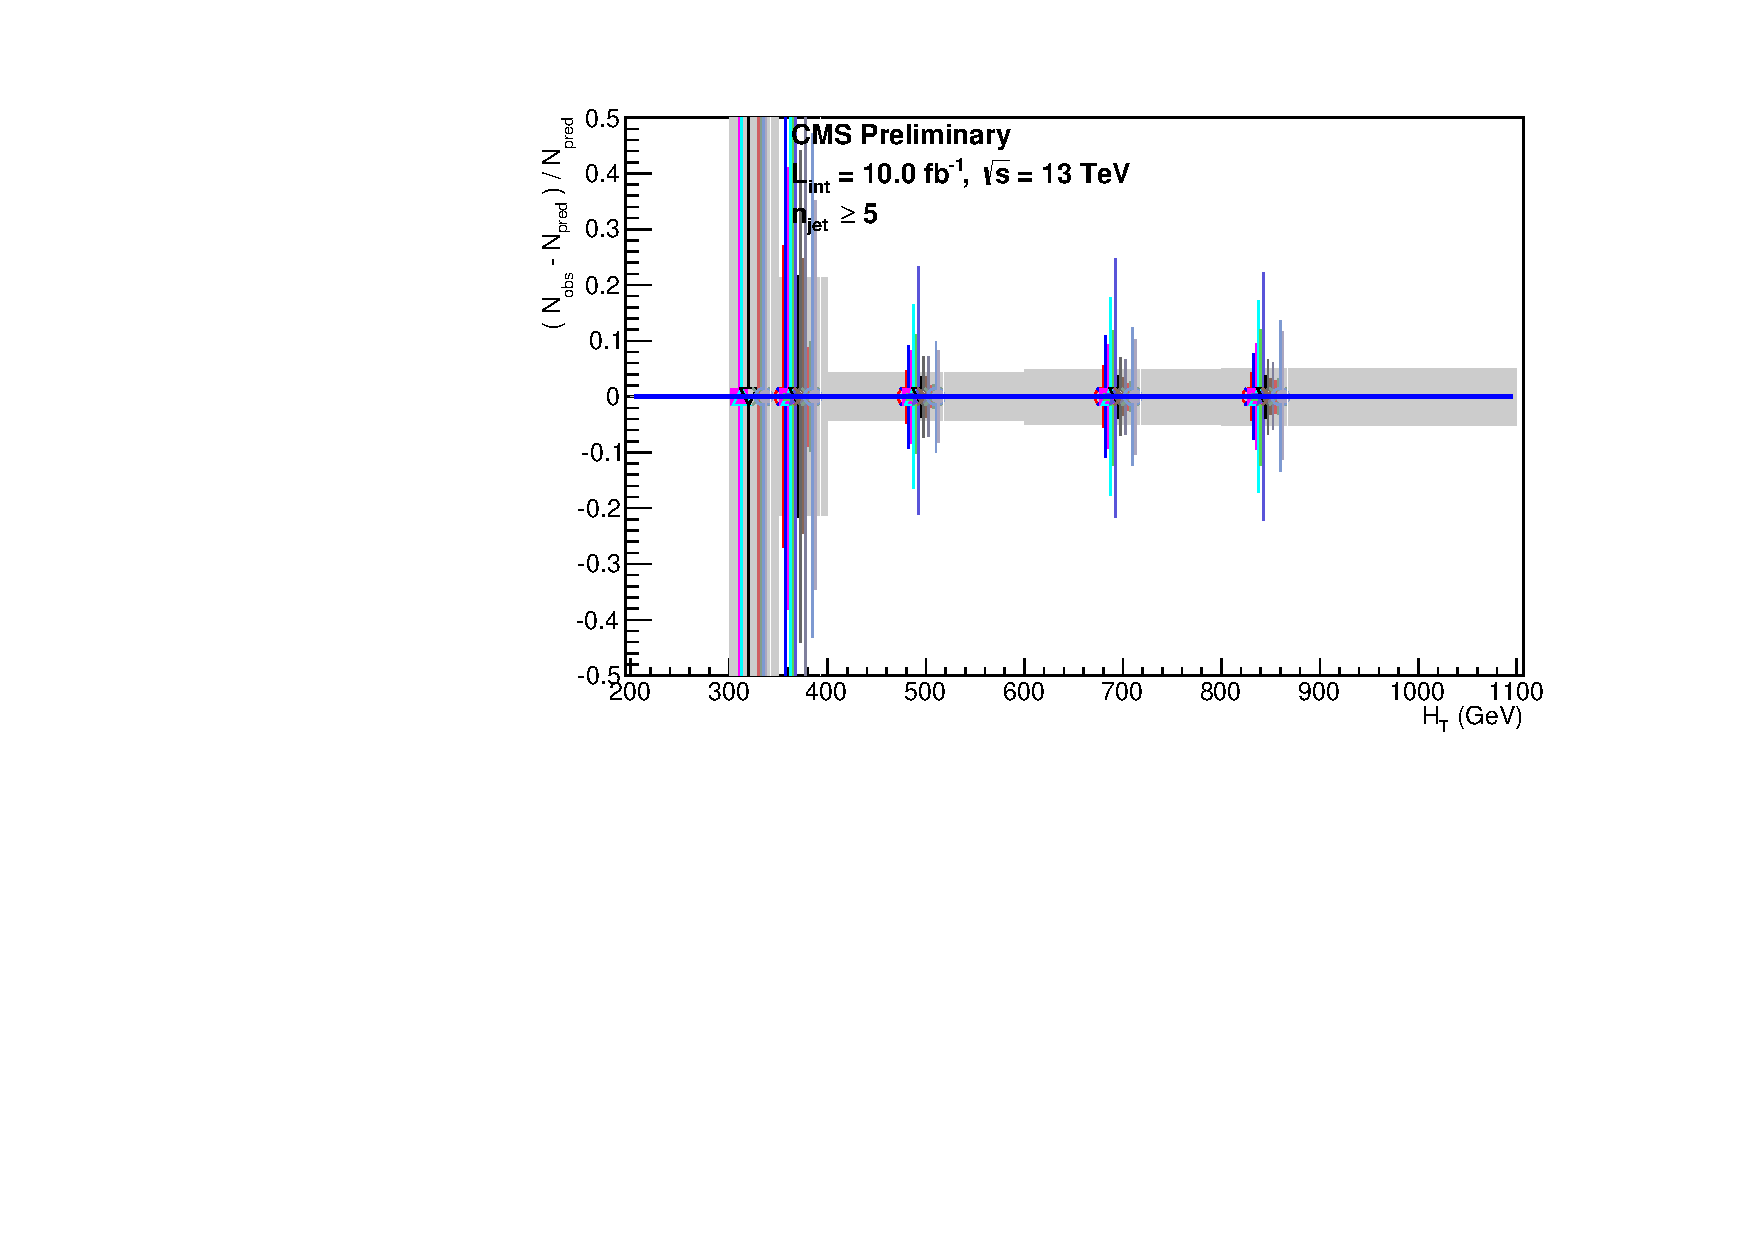
\includegraphics[width=0.5\textwidth]{figures/closureTests/split/Zinv/ge5j_lumi10.pdf}} \\
    \caption{Sets of closure tests chosen to probe the $W$ and \ttbar
      background prediction. Each test is overlaid on top of
      the systematic uncertainty estimates used for each of the seven
      \scalht bins (shaded bands) and for two different jet
      multiplicity bins (columns).}
    \label{fig:ZinvClosure}
  \end{center} 
\end{figure}

A summary of the systematics in each category for the $W$ with \ttbar 
and \znunu transfer factors for two luminosity scenarios are presented in
Figs.~\ref{fig:systematics-ttW} and \ref{fig:systematics-Zinv}
respectively. 

In the $W$ and \ttbar case, the expected systematic errors have decreased 
slightly with respect to those presented in
Sec.~\ref{sec:closure-tests-desc}. As the
closure tests selected for $W$ and \ttbar are now only based on the higher
statistic single lepton control samples, there is a better overall level of
control than when the lower statistic samples were included in the
closure tests used for the systematic error prediction. As the
predicted systematic is a statistical statement about the
extent to which we can say a particular bin is free of bias, we now 
expect this observed lower value. In most bins the
effect is of the order of a few percent.

In the \znunu case, the expected systematic errors have increased with
respect to those presented in Sec.~\ref{sec:closure-tests-desc}. In
this case, many of the selected closure tests contain the lower
statistic single photon and double lepton control samples. The lower
statistics has the opposite effect to that in the $W$ and \ttbar closure 
tests, reducing the level of control and resulting in a larger
expected systematic. In the low jet multiplicity bins the overall
effect is only of the order of a few percent. High jet multiplicity
and low \scalht bins are the most affected. As the \znunu
background is sub-dominant in these cases the overall effect of these
systematic errors is expected to be minor.

% As we observe a small effect when splitting the systematics based on
% the background processes, we chose to not split up the closure
% tests for studies in early data. This keeps it in line with the
% procedure carried out in the $8\tev$ analysis \cite{CMS_AN_2013-366}.

\begin{figure}[]
  \centering
  \subfigure[Systematic uncertainties for 3 \ifb]{
    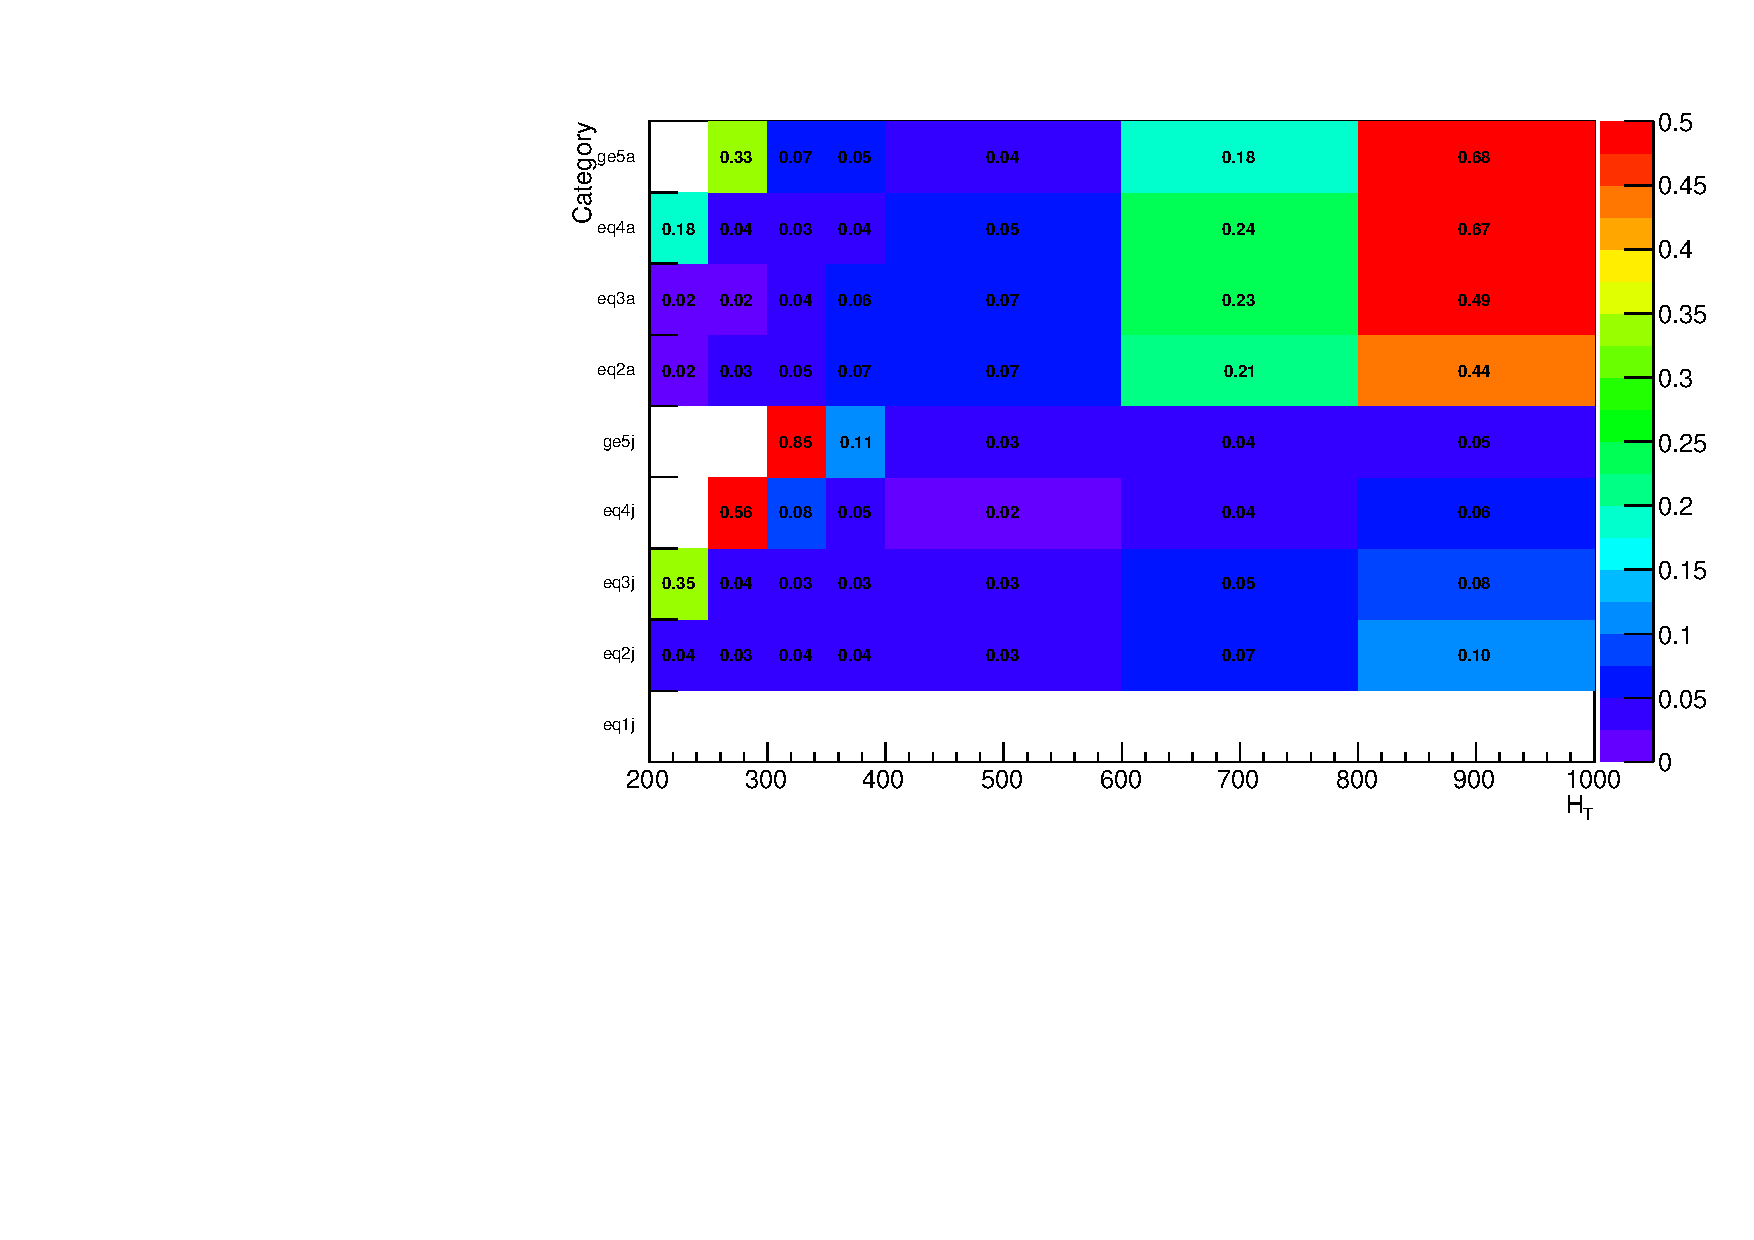
\includegraphics[width=0.8\textwidth]{figures/closureTests/split/ttW/systOut2d3fb.pdf}
  }
%  \subfigure[Systematic uncertainties for 10 \ifb]{
%    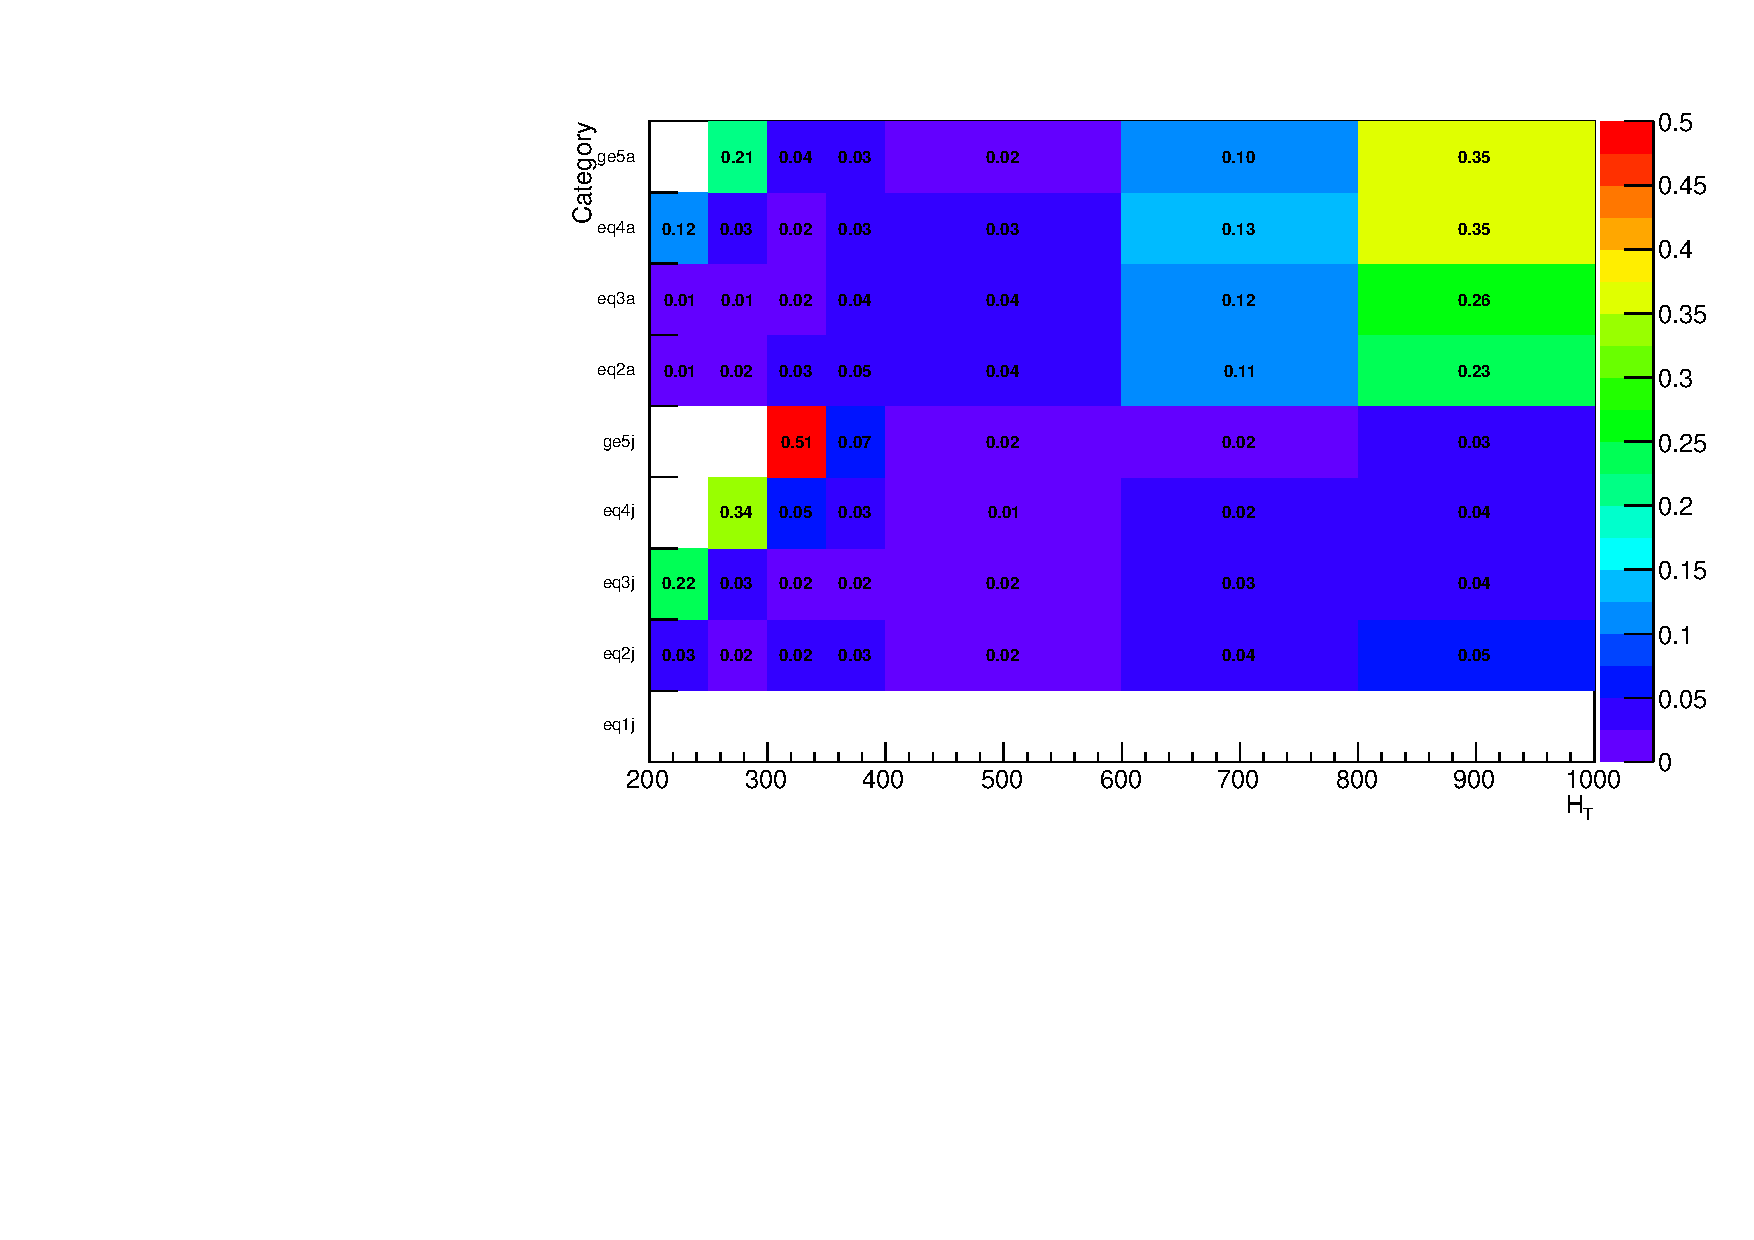
\includegraphics[width=0.5\textwidth]{figures/closureTests/split/ttW/systOut2d10fb.pdf}
%  }
  \caption{\label{fig:systematics-ttW} Expected systematics derived from
  the closure tests selected for the $W$ and \ttbar backgrounds, shown for
  3 \ifb.}
\end{figure}

\begin{figure}[]
  \centering
  \subfigure[Systematic uncertainties for 3 \ifb]{
    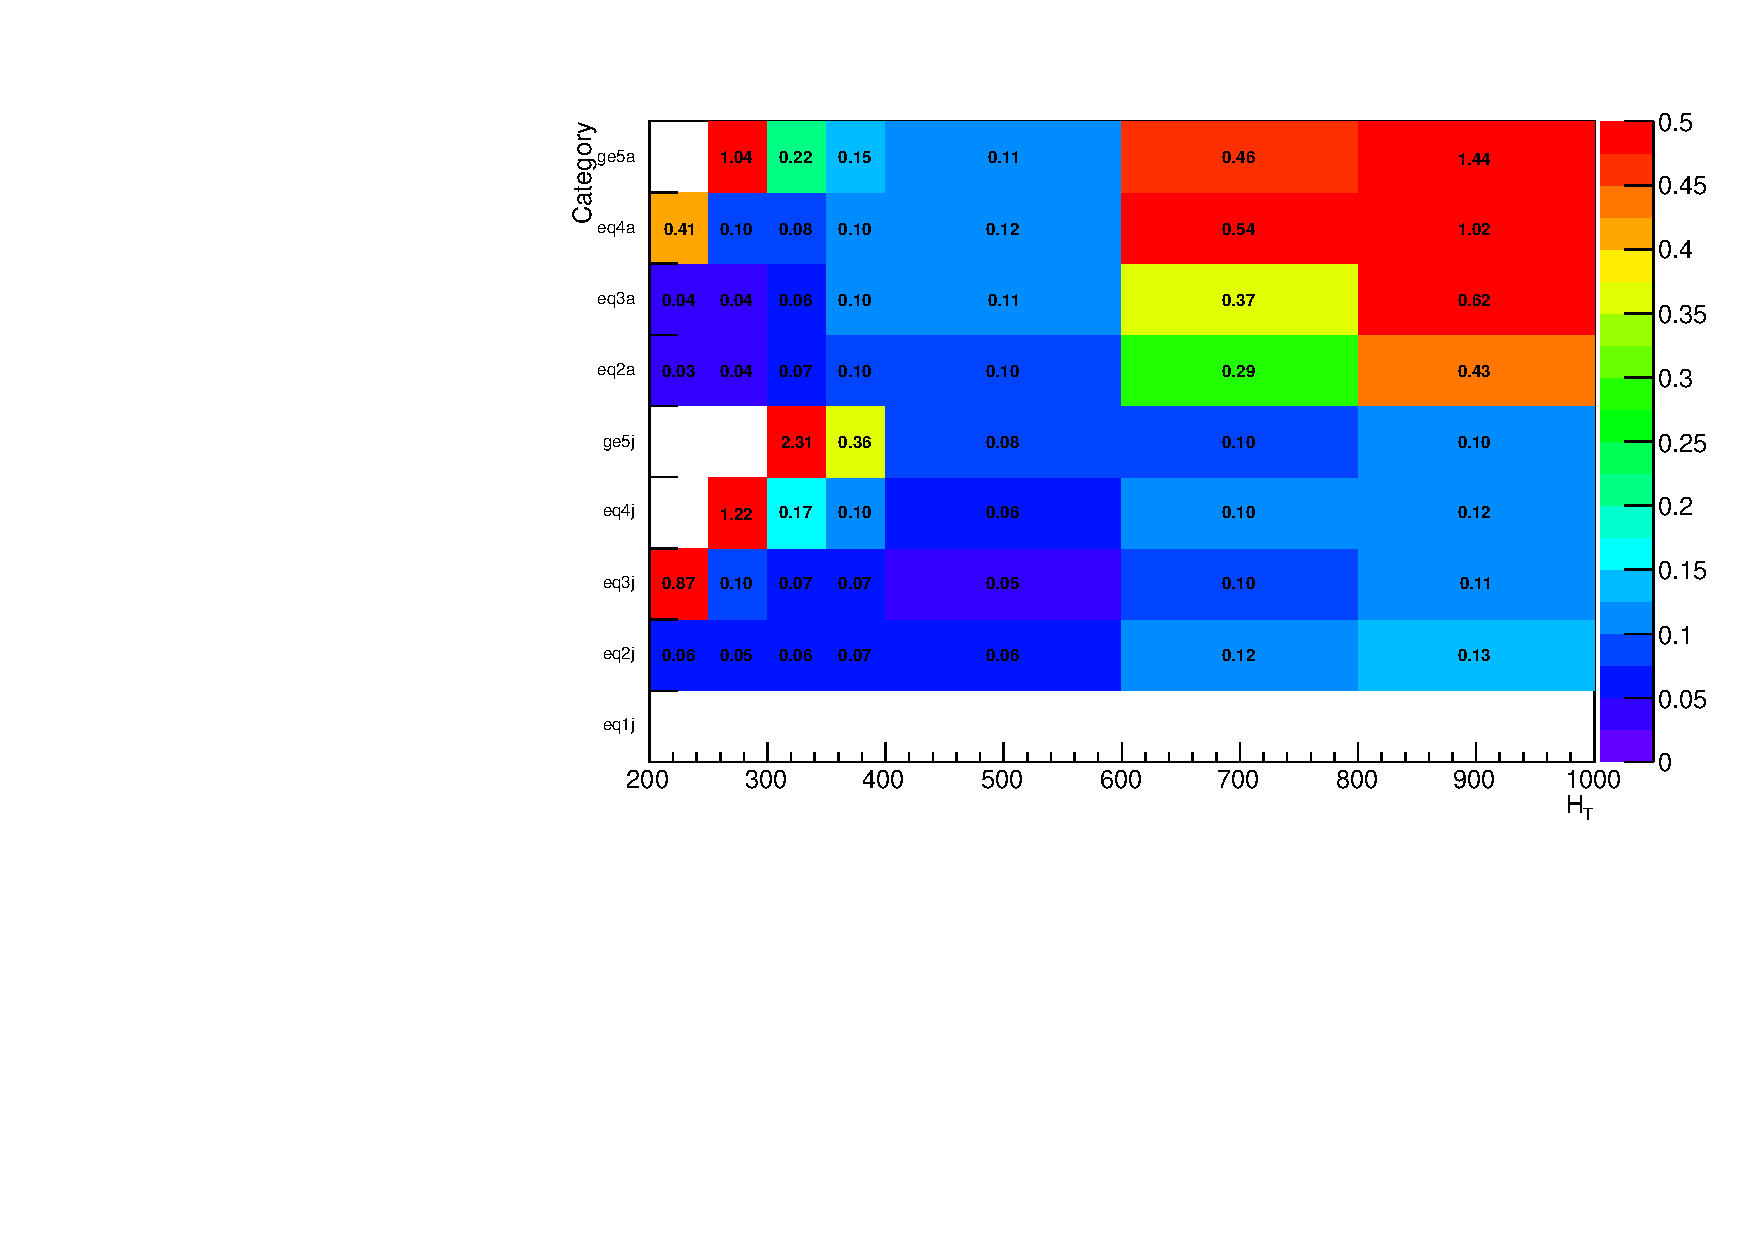
\includegraphics[width=0.8\textwidth]{figures/closureTests/split/Zinv/systOut2d3fb.pdf}
  }
%  \subfigure[Systematic uncertainties for 10 \ifb]{
%    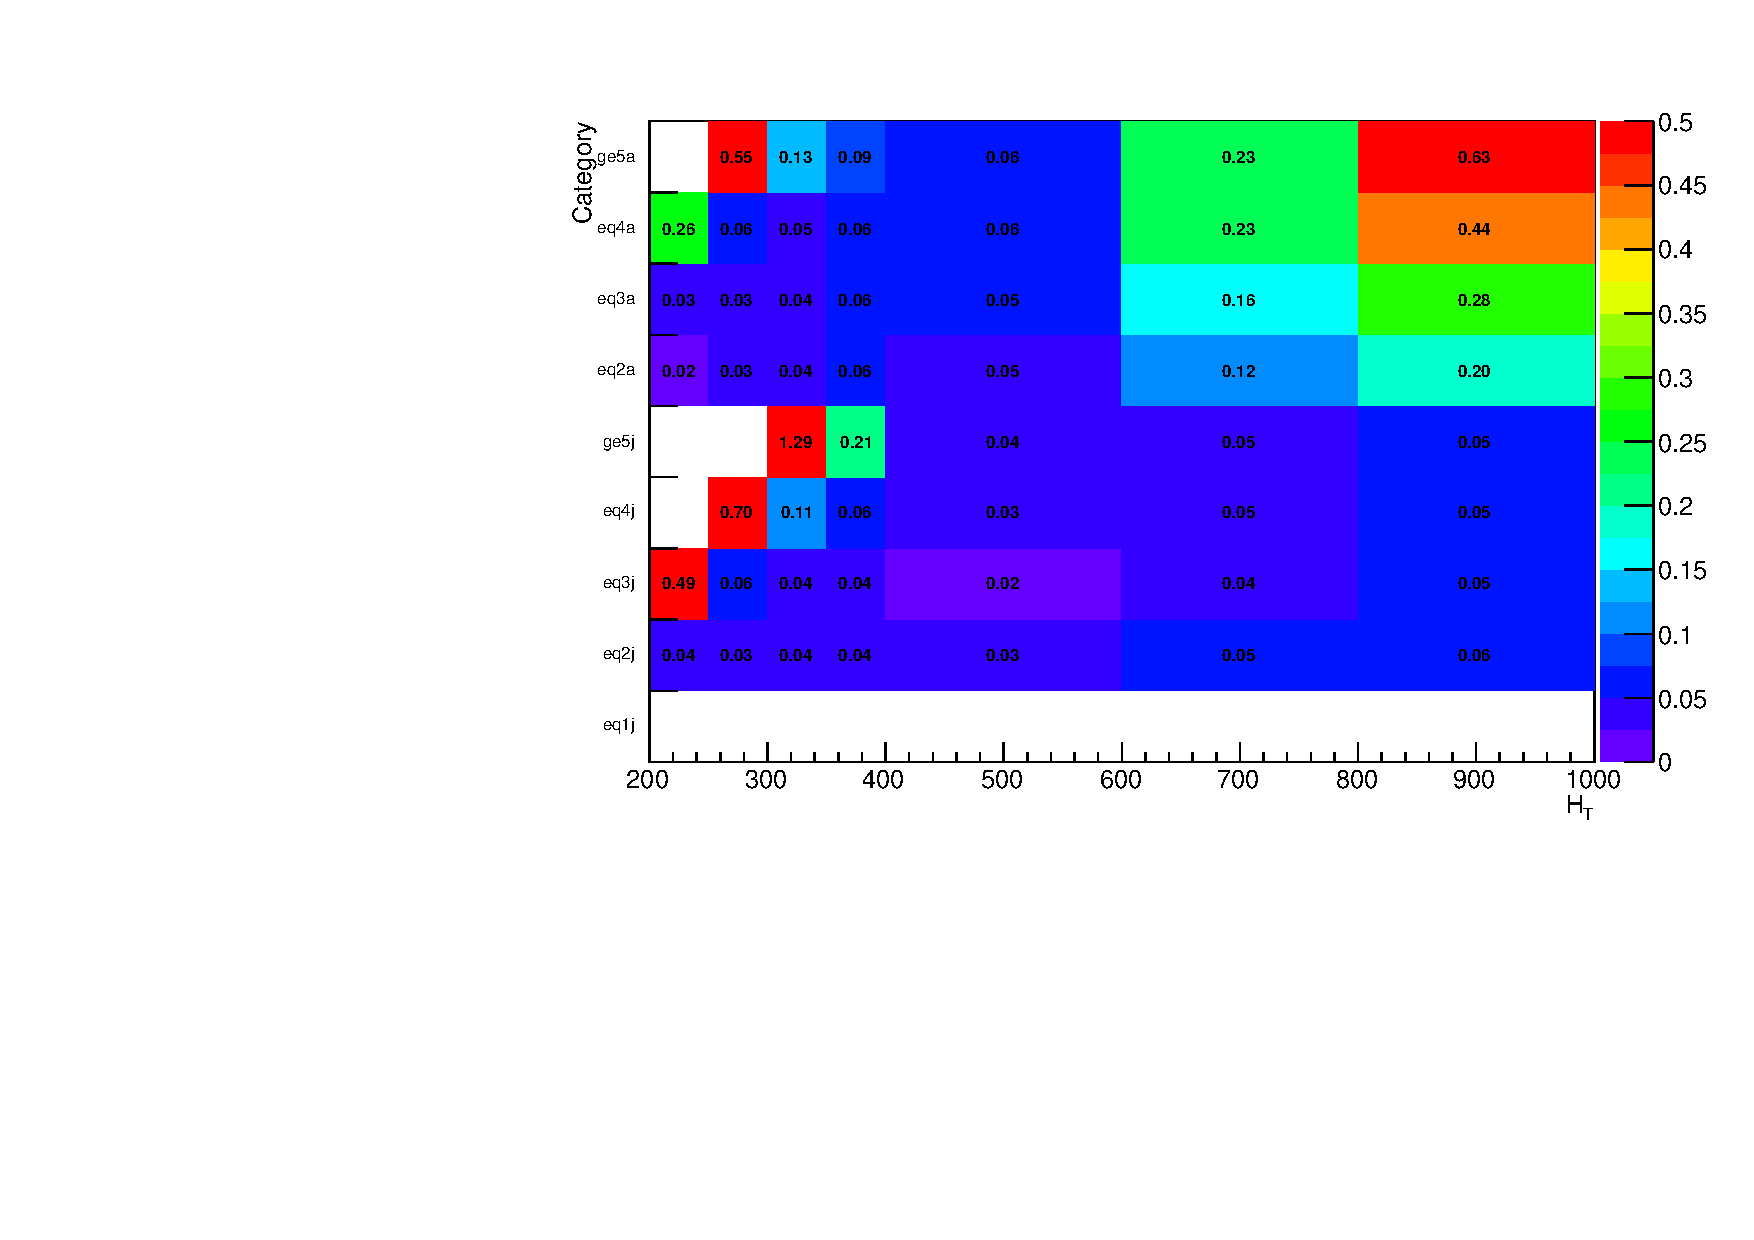
\includegraphics[width=0.5\textwidth]{figures/closureTests/split/Zinv/systOut2d10fb.pdf}
%  }
  \caption{\label{fig:systematics-Zinv} Expected systematics derived from
  the closure tests selected for the \znunu backgrounds, shown for 3 \ifb.}
\end{figure}


